A straightforward way to address dead-salmon artifacts across interpretability methods is to compare findings on a trained target network against a randomized alternative: the same architecture with randomized weights analyzed by the same method. This leads to a principled hypothesis test against a null hypothesis of randomized computation, an idea foreshadowed in early work on probing~\citep{conneau-etal-2018-cram,hewitt-manning-2019-structural,ravichander-etal-2021-probing} and circuit discovery~\citep{shi2024hypothesistestingcircuithypothesis}. We formalize such a test in Appendix~\ref{app:exp} and show that, for probing, it eliminates some false discoveries and substantially reduces effect sizes in standard analyses.

While effective, directly correcting dead-salmon artifacts is a very low bar for interpretability. The goal is to address the deeper statistical issues that give rise to these failures in the first place. Nevertheless, hypothesis testing against computationally meaningful null alternatives naturally motivates a broader statistical–causal reframing of interpretability.

Here, we sketch one such formalization, viewing interpretability as a problem of \emph{statistical–causal inference}. In this view, explanations are \emph{surrogate models} constructed to answer distributions of causal queries about a computational system. An explanation is useful insofar as it supports prediction and manipulation, generalizes under intervention, and remains robust to noise. This perspective aligns with a growing pragmatist approach to interpretability~\citep{P_ez_2019}.

\subsection{Background: Statistical--Causal Inference}

Statistical inference provides the rigorous framework through which empirical observations become scientific knowledge~\citep{cox2006principles,lehmann1998theory}. We argue that interpretability, like every empirical science, must be grounded in these principles. We provide here a brief overview.

\paragraph{Statistical Models and Identifiability.}
A \emph{statistical model} is a family of probability laws $\{\mathbb{P}_\theta^{\bV}:\theta\in\Theta\}$ on a sample space $\mathcal{V}$, indexed by parameters $\theta\in\Theta$. Here, $\bV$ denotes observed data. Intuitively, we assume data arises from some process indexed by unknown parameters~$\theta$, and the goal is to recover~$\theta$ from observations.
% 
Sound inference requires \emph{identifiability}: distinct parameters must induce distinct distributions over observables. Formally, a model is identifiable if $\theta \neq \theta' \implies \mathbb{P}_\theta^{\bV} \neq \mathbb{P}_{\theta'}^{\bV}$. Without identifiability, hypotheses cannot be distinguished from data, rendering inference ill-posed. 

\paragraph{Estimators and Uncertainty Quantification.}
Given finite observations $\mathcal{D}_n=\{\bv^{(i)}\}_{i=1}^n$, an \emph{estimator} $T$ produces an estimate $\hat{\theta} := T(\mathcal{D}_n)$ of unknown parameters $\theta$. Its quality can be assessed through various statistical properties: (i) \textbf{Bias}: Does it recover the correct parameter on average? (ii) \textbf{Variance}: How much does the estimate vary across datasets? (iii) \textbf{Consistency}: Does it converge to the correct parameter as $n\to\infty$? Beyond point estimates, \textbf{confidence sets} provide uncertainty quantification under finite sampling.


\paragraph{Causal Inference.}
Many scientific questions go beyond prediction, seeking explanations of \emph{how} variables influence one another. This requires enriching statistical models with a causal structure~\citep{pearl_causality}.
% 
Let $\bV=\{V_1,\ldots,V_d\}$ denote \emph{endogenous variables}, quantities computed within the system. A directed graph $\mathcal{G}$ over nodes $\bV$ encodes direct causal relationships: an edge $V_i \to V_j$ indicates that $V_i$ directly causes $V_j$. A \emph{structural causal model} (SCM) is the tuple $\mathfrak{C}=(\bV,\bU,\mathbf{f},P_{\bU})$, where:

\begin{itemize}
  \item $\bU$ collects \emph{exogenous} (external) inputs representing unobserved causes or environmental randomness, $P_{\bU}$ is their joint distribution
  \item $\mathbf{f}=\{f_1,\ldots,f_d\}$ are \emph{structural assignments}, functions that deterministically compute each variable from its causes:
\end{itemize}
\begin{equation}
  V_i = f_i(\mathbf{PA}_i, U_i), \qquad i=1,\ldots,d,
\end{equation}
where $\mathbf{PA}_i\subseteq\bV$ denotes the parents of $V_i$ in $\mathcal{G}$, and $U_i\in\bU$ is its exogenous input.

\begin{wrapfigure}{rt}{0.50\textwidth}
    \centering
    \vspace{-1em}
    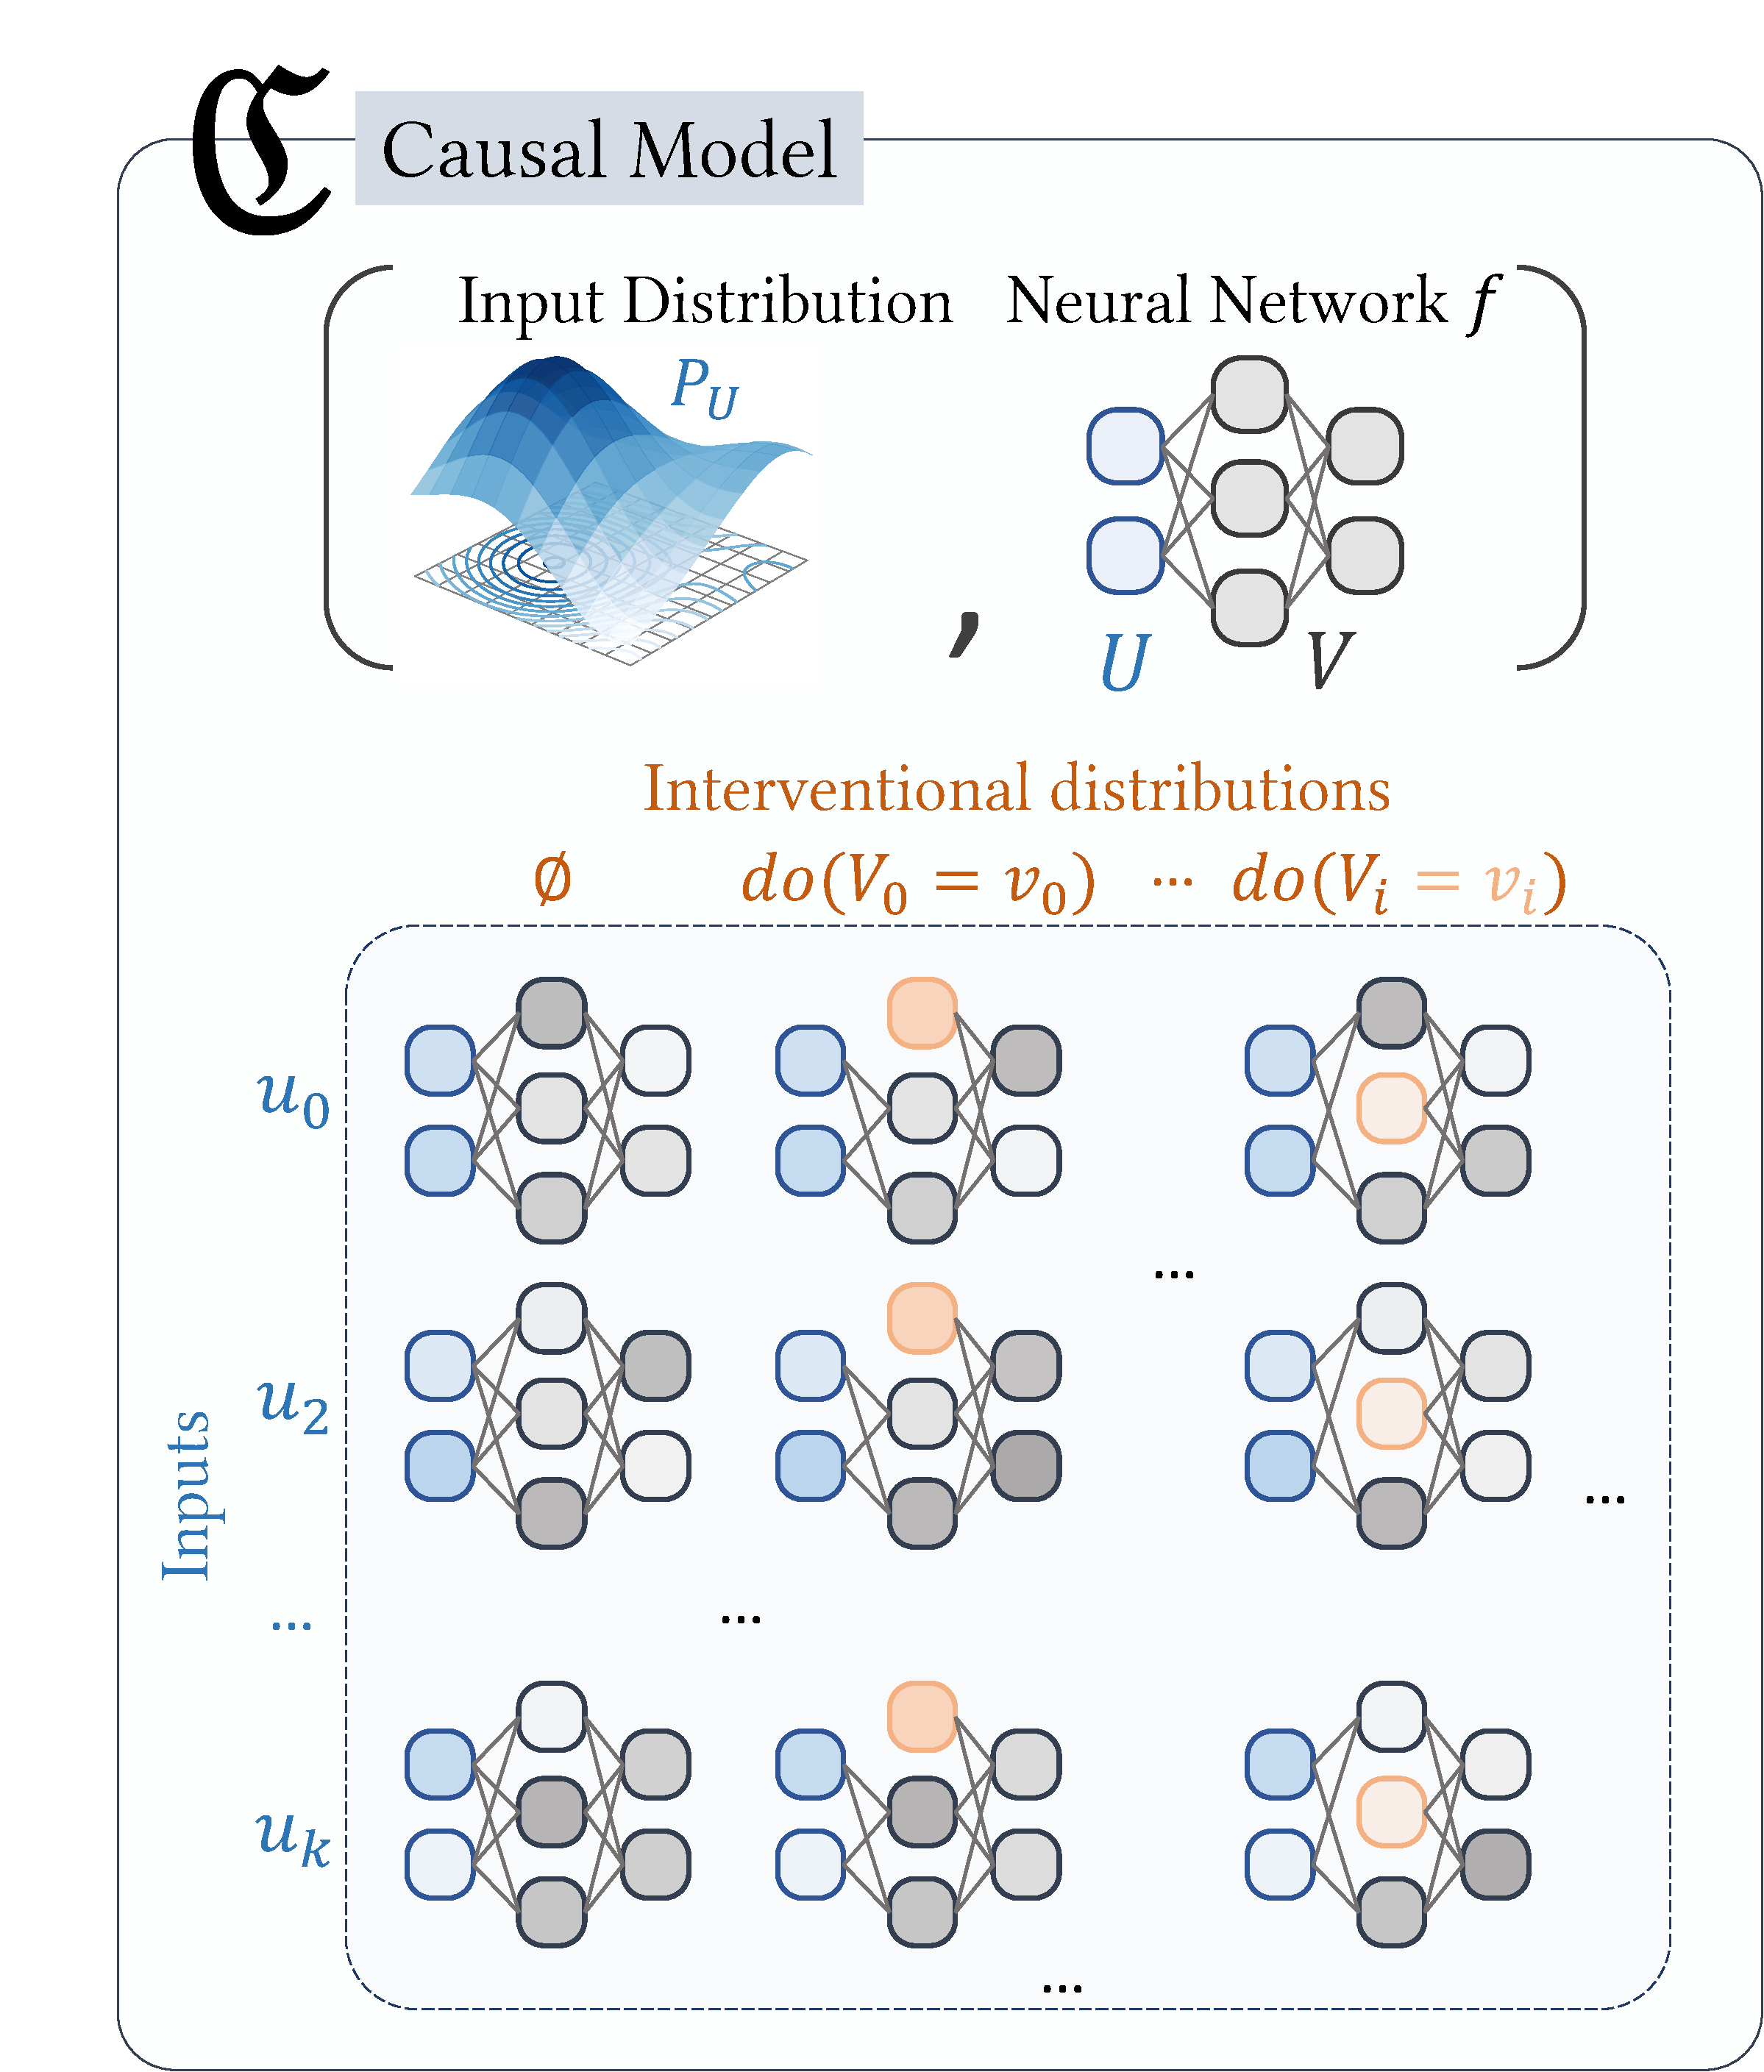
\includegraphics[width=\linewidth]{images/scm_illust.pdf}
    \caption{The tuple of a target behavior $P_{\bU}$ and the computational system with its internal components form an SCM.}
    \label{fig:scm}
    \vspace{-2em}
\end{wrapfigure}



SCMs enable reasoning about interventions and counterfactuals. A \emph{hard intervention} $\mathrm{do}(\bV_I=\bv_I)$ on a subset $\bV_I\subseteq\bV$ replaces the structural assignments for variables in $\bV_I$ with constants $\bv_I$, overriding their causal mechanisms. The intervened model $\mathfrak{C};\mathrm{do}(\bV_I=\bv_I)$ induces an \emph{interventional distribution} $P^{\mathfrak{C};\mathrm{do}(\bV_I=\bv_I)}_{\bV}$, which captures how the system behaves under this external manipulation.

A \emph{causal query} $q(\mathfrak{C})$ is any well-defined question about the SCM, such as ``What is the marginal distribution of $V_i$?'' or ``What is the average effect of setting $V_i=v$ on outcome $V_m$?'' Thus, a causal query is any measurable functional of the SCM, possibly involving conditioning or intervention. Central to causal inference is \emph{query identifiability}: whether $q(\mathfrak{C})$ can be uniquely determined from available observational or interventional data.


\subsection{Neural Networks as Structural Causal Models}
Returning to modern AI interpretability, we first state a standard framing of computational systems as SCMs. Let $f$ be a computational system, typically a neural network, with internal computational elements $\bV$ and input distribution $P_{\bU}$. The input distribution $P_{\bU}$ represents the \emph{behavior of interest} that we aim to explain. For instance, $P_{\bU}$ might represent arithmetic prompts to a language model, images from a particular domain, or factual questions about a specific topic.

The tuple $(f, P_{\bU})$ naturally defines an SCM $\mathfrak{C} = (\mathcal{G},\; \bV,\; \bU,\; \mathbf{f},\; P_{\bU})$, where:
\begin{itemize}
  \item \textbf{Endogenous variables} $\bV$ are the network's computational variables (e.g., hidden states, attention patterns, outputs).
  \item \textbf{Exogenous variables} $\bU$ are inputs sampled from $P_{\bU}$, representing the behavior we seek to explain.
  \item \textbf{Structural assignments} $\mathbf{f}$ are the deterministic functions defining the network's computation (layers, attention mechanisms, nonlinearities).
  \item \textbf{Causal graph} $\mathcal{G}$: the network's computation graph.
\end{itemize}

The SCM induces a unique \emph{observational distribution} over $\bV$: sampling corresponds to drawing inputs from $P_{\bU}$, executing a forward pass, and recording desired activations. Also, the SCM encodes \emph{interventional} and \emph{counterfactual} distributions based on external modifications of the inner computation.
This perspective is standard within mechanistic interpretability~\citep{olah2018the,cammarata2020thread,pmlr-v162-geiger22a,geiger2025causalabstractiontheoreticalfoundation} and is illustrated in Figure~\ref{fig:scm}. Then, a \emph{causal query} is any well-specified quantity about $\mathfrak{C} := (f, P_{\bU})$, such as ``What distribution would the network produce if we forced activation $V_i$ to value $v$?'' or ``How much does attention head $V_a$ causally contribute to correct factual recall?''



\subsection{Explanations as Surrogate Models}

In an attempt to provide a general statistical-causal perspective on interpretability, we formalize explanations as \emph{surrogate models}: simpler computational descriptions designed to answer chosen collections of causal queries about a target system. This perspective treats interpretability as a form of model compression, where we seek a simpler model that faithfully approximates a complex system's behavior for queries we care about. In this perspective, every interpretability method is characterized by three ingredients:
\begin{enumerate}
  \item \textbf{Query space} $Q$ with \textbf{distribution} $\mu$: The set of causal queries to be answered by the explanation. It dictates what aspects of $\mathfrak{C}$ should be explained. This encodes our explanatory goals.
  \item \textbf{Surrogate class} $\mathcal{E}$: The class of admissible explanations. It dictates what forms the explanation can take, e.g., circuits, sparse subgraphs, linear probes, concept vectors, causal graphs, \dots
  \item \textbf{Discrepancy measure} $D$: How we measure whether a surrogate (member of $\mathcal{E}$) \textit{correctly} answers queries.
\end{enumerate}
This framework is (non-rigorously) illustrated with the example of circuit discovery in Figure~\ref{fig:framework}.
% 
While standard causal inference often concentrates $\mu$ on a \emph{single} causal query (e.g., average treatment effect), interpretability aims to answer \emph{many diverse queries} drawn from a non-trivial distribution $\mu$.
For example, $\mu$ might distribute probability over interventional queries and counterfactual queries across network components, or any functionals of the interventional and counterfactual distributions. 
% Answering such queries requires the hypothesis class to be more complex than real number parameters. 



For instance, we can view each candidate explanation $e \in \mathcal{E}$ as defining a \emph{query-answering map} $S_e: Q \to \mathcal{R}$, where $S_e(q)$ is the surrogate's predicted answer to query $q$, and $\mathcal{R}$ is the space of possible answers for query $q$ (e.g., probability distributions, scalar effects, or discrete predictions). The surrogate's \emph{fidelity} is measured by the discrepancy function $D: \mathcal{R} \times \mathcal{R} \to \mathbb{R}_+$ quantifying the error between the answer from $q(\mathfrak{C})$ and the surrogate's prediction $S_e(q)$.
% 
Then, we can define the \emph{population risk} of a candidate explanation as the expected error over queries:
\begin{equation}
\label{eq:population_risk}
L_\mu(e) = \mathbb{E}_{q\sim\mu}\big[D\big(q(\mathfrak{C}),\, S_e(q)\big)\big].
\end{equation}
An ideal explanation $e^* \in \mathcal{E}$ minimizes this risk: $e^* \in \arg\min_{e \in \mathcal{E}} L_\mu(e)$.



% Each explanation $e$ from the hypothesis space $\mathcal{E}$ can be seen as defining a \emph{query-answering map} $S_e$, where $S_e(q)$ is the surrogate's predicted answer for query $q$.

% To measure fidelity, choose an error measure $D$ and define a \emph{population risk}:
% \begin{equation}
% \label{eq:population_risk}
% L_\mu(e) = \mathbb{E}_{q\sim\mu}\big[D\big(q(\mathfrak{C})\,\|\,S_e(q)\big)\big].
% \end{equation}

\begin{figure}
    \centering
    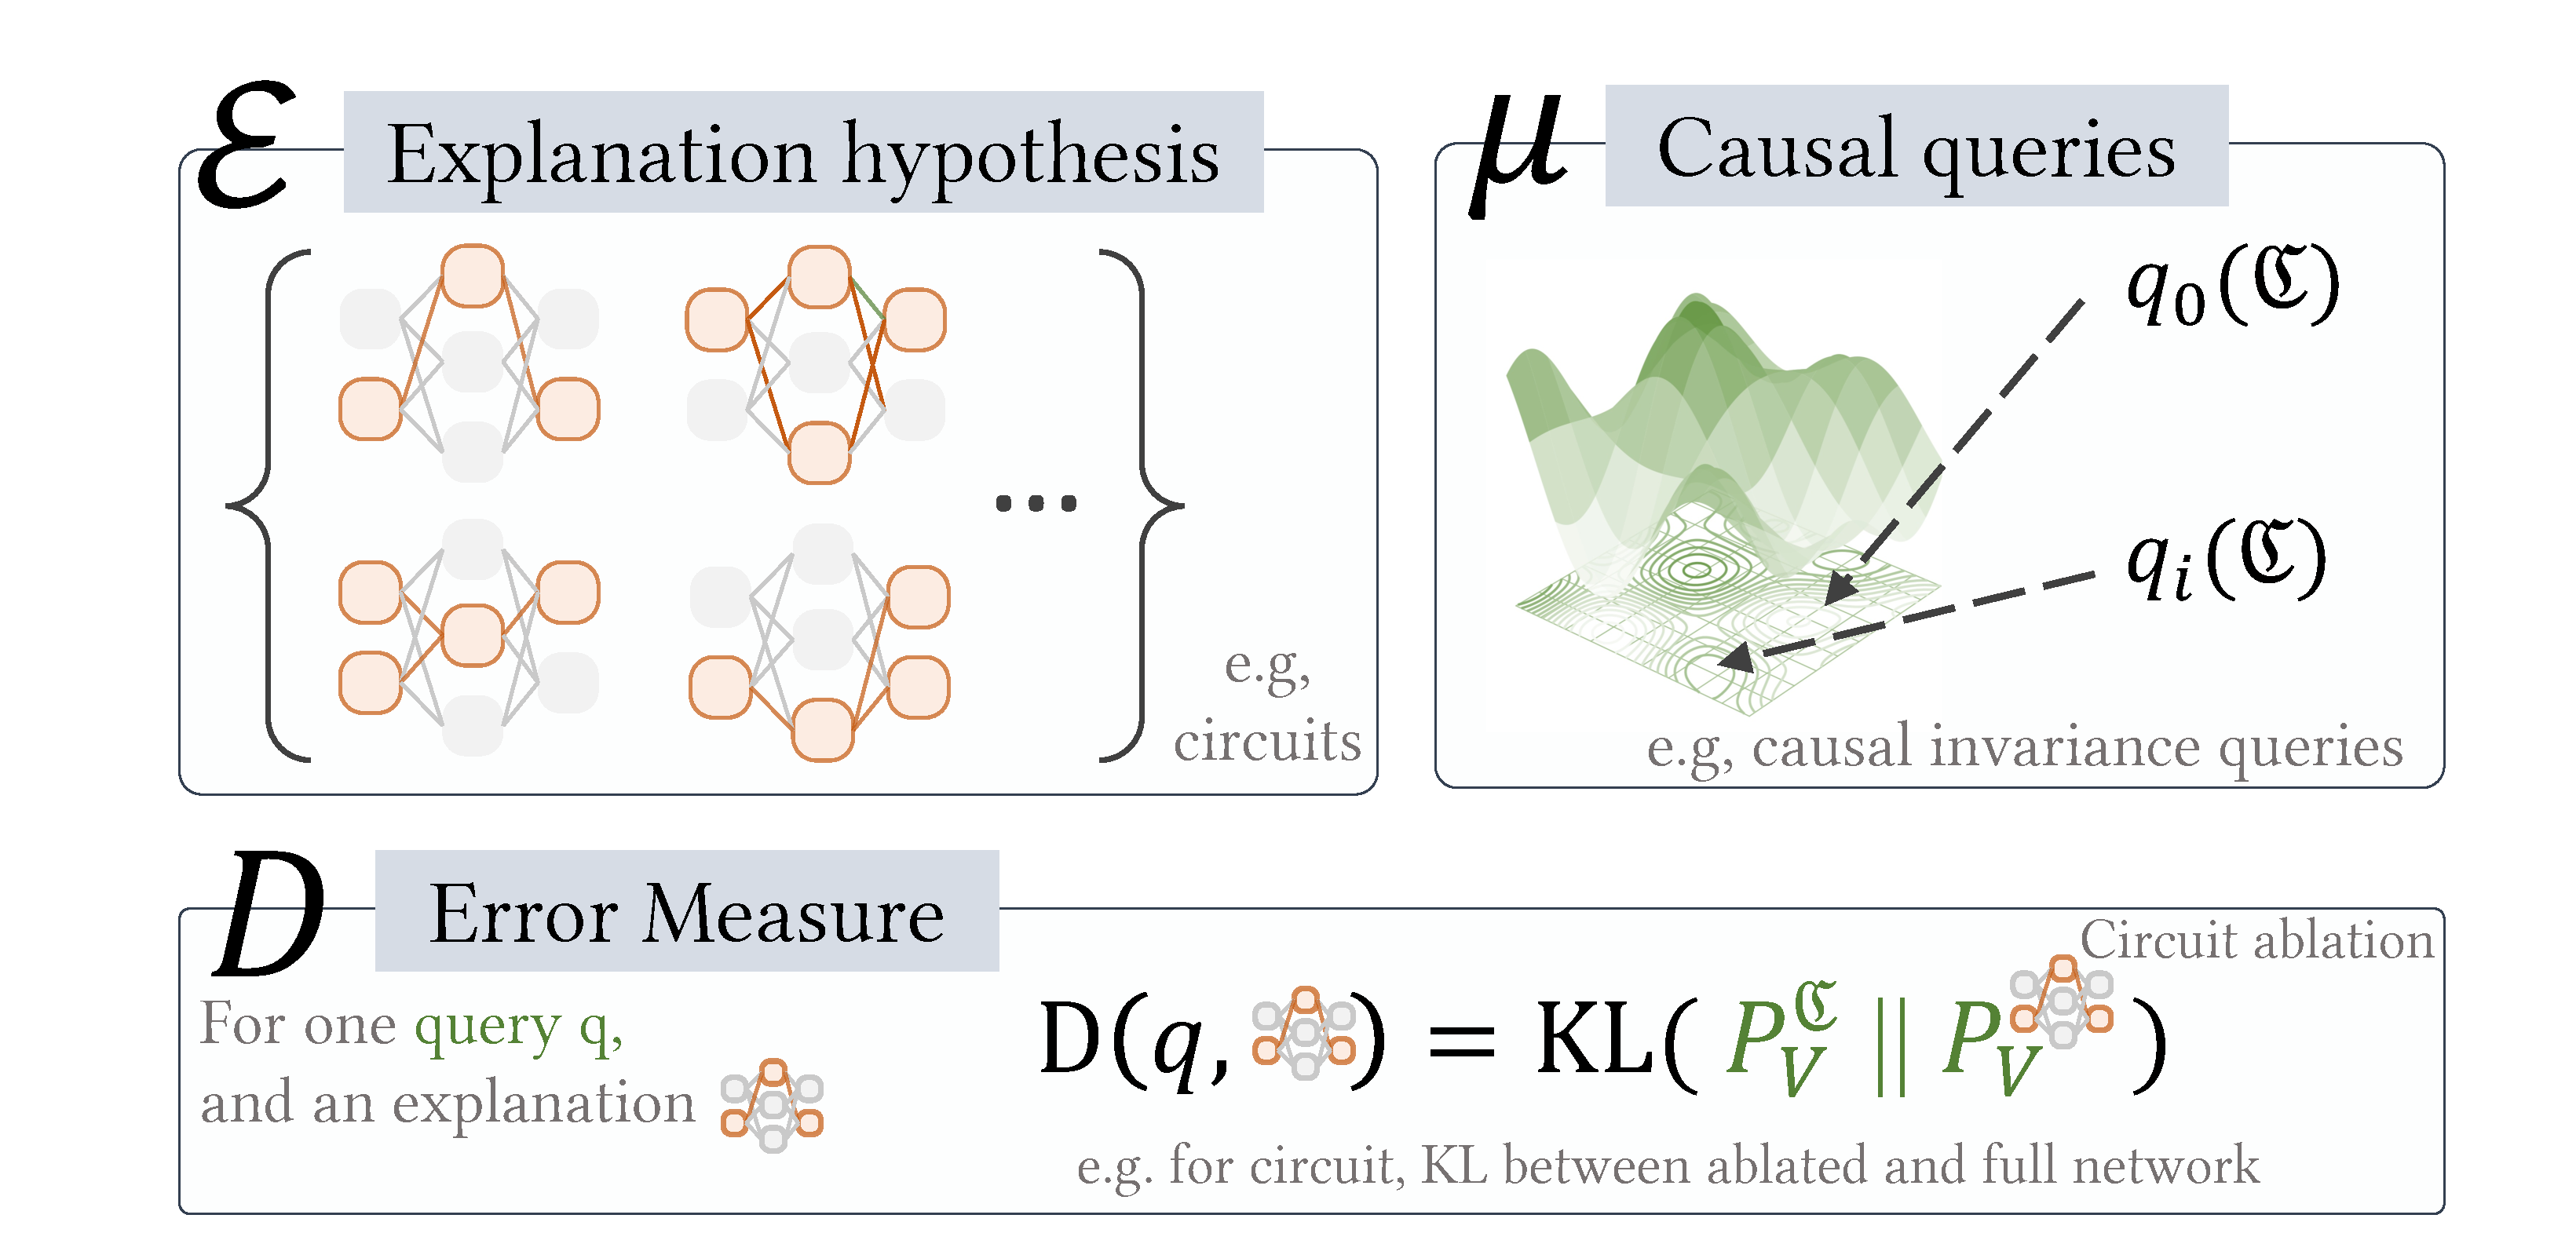
\includegraphics[width=0.8\linewidth]{images/framework_illust.pdf}
    \caption{An interpretability task is defined by three elements: $\mathcal{E}$, the hypothesis space; $\mu$, the distribution over causal queries about the SCM (model and behavior); and $D$, the error measure.}
    \label{fig:framework}
\end{figure}

\paragraph{Interpretability Task and Identifiability.}
We call the triple $(\mu, \mathcal{E}, D)$ an \emph{interpretability task}, fully specifying what we aim to explain (query distribution $\mu$), what explanations are admissible (hypothesis class $\mathcal{E}$), and how we measure success (discrepancy $D$).
% 
The task is \emph{identifiable} if $L_\mu$ admits a unique minimizer in $\mathcal{E}$ (potentially up to predefined acceptable symmetries). Identifiability captures whether the surrogate class can, in principle, be distinguished using the queries deemed relevant by $\mu$. Without identifiability, multiple incompatible explanations achieve the same population risk, making inference fundamentally ambiguous. The analysis of Section~\ref{sec:description} indicates that the most common tasks are not identifiable.
% 
Finally, this reframing highlights that explanations are \emph{pragmatic computational summaries} of the structure encoded by $\mathfrak{C} := (f, P_{\bU})$. They are inferred models useful for specific explanatory purposes. 

% The interpretability task is the tuple $(\mu, \mathcal{E}, D)$ specifying query distribution, surrogate hypothesis space, and error measurement. The task is \emph{identifiable} if $L_\mu$ admits a unique minimizer in $\mathcal{E}$ (up to allowed symmetries). Identifiability captures whether the surrogate class can, in principle, be distinguished using queries deemed relevant by $\mu$. Crucially, this highlights that explanations are \emph{computational summaries} of the computational structure encoded by $\mathfrak{C} := (f, P_{\bU})$.
% 
% This reframing is not superficial application of statistical tools to interpretability outputs. It proposes viewing interpretability as \emph{inference of structured objects} (explanations) from computational traces.

\paragraph{Estimation with Finite Data.}
In practice, we face two types of finite sampling difficulties. First, we observe only finitely many queries $q_1,\ldots,q_n \sim \mu$ from the query distribution. Second, for each query $q_j$, we can only collect a finite amount of computational traces by sampling inputs $\bU \sim P_{\bU}$ and recording the corresponding activations and outputs, potentially under interventions.
% 
Let $\mathcal{T}_n$ denote the complete dataset of query-trace pairs. An interpretability method $M$ acts as an \emph{estimator}, mapping this finite dataset to an estimated surrogate explanation:
\begin{equation}
\hat{e} := M(\mathcal{T}_n).
\end{equation}
A natural estimator is given by empirical risk minimization: choose $\hat{e}$ to minimize the empirical risk $\widehat{L_\mu}(e) = \frac{1}{n}\sum_{j=1}^n \widehat{D}(q_j(\mathfrak{C}) ,\, S_e(q_j))$, where $\widehat{D}$ is estimated from finite traces.
% 
% Finite-sample uncertainty about the estimate arises from \emph{both} levels of sampling: (i) \textbf{Trace sampling uncertainty}: For each query $q_j$, estimates of $q_j(\mathfrak{C})$ and $D(q_j(\mathfrak{C}) , \, S_e(q_j))$ rely on finite samples from $P_{\bU}$. (ii) \textbf{Query sampling uncertainty}: The empirical risk $\widehat{L_\mu}$ is estimated over finite queries.

% When $\mu$ concentrates on a single query, standard tools (law of large numbers, central limit theorem) provide consistency guarantees and confidence intervals. However, when $\mu$ has broad support over many queries, both sources of uncertainty compound. Key open questions emerge: How should we quantify total uncertainty in estimated explanations? How many queries and traces suffice for reliable inference? Can we optimally select which interventional data to collect to maximize information about $\mathcal{E}$? 
Relevant to this exposition, \citet{pmlr-v202-senetaire23a} proposed a statistical framing for feature attribution. Then, previous works already explored hypothesis testing and uncertainty quantification for circuit discovery~\citep{shi2024hypothesistestingcircuithypothesis,meloux2025mechanisticinterpretabilitystatisticalestimation}.


\subsection{Re-Interpreting Documented Issues}
The framework does not prescribe which $(\mu, \mathcal{E}, D)$ researchers should adopt. Rather, it provides a \emph{shared language} for making assumptions explicit and rooted in the tools of statistical inference. Different research programs will choose different hypothesis classes or query distributions; the framework ensures that such choices are transparent and their implications are analyzable. Table~\ref{tab:interpretability_methods} in the appendix illustrates how existing interpretability methods can be mapped into this formulation, each implicitly making assumptions about queries, surrogates, and error metrics. Under this view, the issues described in Section~\ref{sec:description} can be understood as problems of \emph{non-identifiability}.

\paragraph{Behavioral Benchmarks.}
Benchmarks that evaluate model outputs against a gold standard (averaged success over input distributions) ask an identifiable question: \textit{how well does the model perform under a specific task distribution and error metric?} This is arguably the simplest form of interpretability and drove most of the progress in AI. Its usefulness depends on the construction of the benchmark, but the inference problem is well-posed.

\paragraph{Concept-Based Approaches.}
Predictive methods (probes, SAEs) inherit non-identifiability issues from the underlying underspecification of machine learning tasks~\citep{10.5555/3586589.3586815}.
For example, methods like Concept Activation Vectors~\citep{kim2018interpretability, cunningham2023sparseautoencodershighlyinterpretable} postulate that internal states $\bv$ are generated by interpretable concepts $\mathbf{z}$ via $\bv = g(\mathbf{z})$.
This is an instance of (causal) representation learning, which is \textbf{non-identifiable} without auxiliary information \citep{Locatello2019, Khemakhem2020}. 
It is therefore unsurprising that proposed improvements mirror standard remedies for underspecification in machine learning: regularization in the form of capacity control for probes~\citep{belinkov-2022-probing} or cross-validation to assess generalization~\citep{kantamneni2025sparseautoencodersusefulcase}.

% \paragraph{Feature Attribution.}
% Attribution methods (e.g., Integrated Gradients) explain predictions relative to a baseline input $\tilde{\bx}$. The query is effectively: "How does the output change as we interpolate from $\tilde{\bx}$ to $\bx$? This task is \textbf{non-identifiable} because the explanation strictly depends on $\tilde{\bx}$, yet the "correct" baseline for natural data is undefined. Different baselines yield valid but contradictory attribution maps \citep{sturmfels2020visualizing}, meaning that the attribution is not uniquely determined by the computational traces alone.

\paragraph{Causal Mediation Analysis.}
Methods like causal mediation analysis \citep{meng2022locating, vig2020causalmediationanalysisinterpreting} estimate the indirect effect of a component on observed outputs. As the intervention and model are fully specified, the mediation estimand is unique and \textbf{identifiable}. However, the explanatory claim that a component with high effect is the \textit{locus} of a mechanism is \textbf{not identifiable}, because of the overdetermined causal structure. 
% Furthermore, causal mediation analysis requires the choice of a destructive intervention to estimate the indirect effect. There is no consensual way to choose this intervention and different choices lead to different results~\citep{meloux2025mechanisticinterpretabilitystatisticalestimation}.

\paragraph{Circuit Discovery and Causal Approaches.}
Circuit discovery seeks a subgraph $G' \subset G$ that preserves the model's performance. This task faces the "Hydra effect" \citep{mcgrath2023hydraeffectemergentselfrepair} and causal overdetermination. If parallel pathways $A$ and $B$ are sufficient, circuits containing only $A$ or only $B$ both satisfy fidelity criteria. Thus, even \textit{correct} causal methods may recover many different explanations consistent with the same behavior \citep{melouxeverything}. Addressing this requires formulating identifiable causal questions. Causal abstraction \citep{Beckers_Halpern_2019,geiger2025causalabstractiontheoreticalfoundation} offers a promising direction, as it operates at a coarser representational level where overdetermination can be absorbed into the abstracted representations. However, current operational metrics demonstrate empirical non-identifiability~\citep{melouxeverything, sutter2025nonlinearrepresentationdilemmacausal}.

% \paragraph{Natural Language Explanations.}
% Methods that prompt LLMs to generate their own explanations (e.g., Chain-of-Thought) treat the explanation space $\mathcal{E}$ as the set of all possible natural language strings. Since the explanation generation is often separate from the prediction pathway, there are infinitely many semantic strings that are plausible to a human but causally unfaithful \citep{turpin2023languagemodelsdontsay}.
% This task therefore suffers from extreme \textbf{non-identifiability}: in the space of language, the "rationalization gap" allows for explanations that are semantically disjoint while maintaining high likelihood.

% These questions parallel optimal experimental design in statistics. Experimentalists msut choose which treatments to randomize, and interpretability researchers must choose which interventions to perform on neural networks.

% In practice, we observe finite queries $q_1,\ldots,q_n\stackrel{\text{i.i.d.}}{\sim}\mu$, collecting finite computational traces per query by sampling inputs from $P_{\bU}$. Let $\mathcal{T}_n$ denote the resulting dataset. An interpretability method $M$ acts as an estimator mapping $\mathcal{T}_n$ to estimated surrogate $\hat{e} := M(\mathcal{T}_n)$. A natural approach would be to choose the estimator that minimizes the \emph{empirical risk} $\widehat{L_\mu}(e)$.
% 
% Finite-sample uncertainty arises from both query sampling and finite inputs per query.
% When $\mu$ is concentrated on a single query, the standard tools of the law of large number give consistency guarantees (convergence in  $\mathcal{E}$ as the number of observations grows) and methods to estimate uncertainty. However, when $\mu$ is non-trivial, uncertainty also arises from non-exhaustive sampling of queries. A key question becomes: how to quantify uncertainty in these scenario and how to choose interventional data on the computational sysmte to quickly converge to a confident explanation.

% \paragraph{Interpretation of Common Methods.}


% By making these choices explicit, we can ask: Which tasks are identifiable? What are their sample complexity requirements? When do methods fail, and why? The failure modes documented in the previous section suggest that most approaches suffer from non-identifiability.

% Importantly, this framework is \emph{normatively neutral}. It does not prescribe which $(\mu, \mathcal{E}, D)$ researchers ought to study. Rather, it provides a \emph{lingua franca} for specifying assumptions, comparing methods, and critically evaluating claims. Different research programs may instantiate vastly different hypothesis classes; the framework ensures these choices are transparent and comparable. Table~\ref{tab:interpretability_methods} describes how common methods instantiate this framework.

% \paragraph{Takeaway.}
% Viewing interpretability as constructing surrogates that approximate distributions of causal queries makes explicit the implicit choices practitioners face: which queries matter ($\mu$), how closely they must match ($D$), and what surrogates are admissible ($\mathcal{E}$ and regularization). This perspective brings the full apparatus of statistical and causal inference---estimands, identifiability, risk, finite-sample error---to interpretability research. Conceptually, it reveals explanation as \emph{computational compression}: surrogates compress aspects of network computation encoded by query distribution $\mu$. comparable rather than implicit.




% To make progress, we advocate adopting a pragmatist and instrumentalist perspective. The central question becomes not whether an explanation corresponds to some metaphysically privileged ground truth, but whether it is useful: predictive, manipulable, generalizable under intervention, and resilient to noise. Such a shift sidesteps metaphysical debates and centers methodology on empirical utility. This naturally motivates a statistical inference framework. Modern empirical sciences resolved analogous problems by explicitly formulating explanations as estimands, embedding them in statistical models, and quantifying uncertainty.

% In the remainder of this section, we introduce one possible formalization that embodies these principles for AI interpretability.
% Importantly, the statistical--causal inference framework does not dictate any particular normative commitments about which classes of explanations researchers ought to study. It merely provides a lingua franca for specifying assumptions, comparing methods, and critically evaluating claims. Different research programs may instantiate very different hypothesis classes, statistical models, with varying identifiability criteria. The framework ensures these choices are transparent rather than implicit.

% \subsection{Preliminaries}
% Let $\mathbf X$ denote the random input to a neural network (e.g.\ tokens in language models or pixels in vision models). We represent the network as a directed acyclic graph (DAG)
% \(f:\mathcal X\to\mathcal Y\), whose nodes correspond to computational units (neurons, channels, or other units of computation) and whose directed edges encode information flow determined by parameterized maps (weights).

% Formally, let $\mathbf V$ be the set of nodes in the computation graph $\mathcal G$, including the designated output node(s) $Y\in \mathbf V$. Each node $v\in \mathbf V$ computes a measurable function of its parents $\mathrm{pa}(v)\subset \mathbf V$, parameterized by weights $W_v$:
% \[
% h_v \,=\, g_v\big(\{h_u:\; u\in\mathrm{pa}(v)\},\; W_v\big), \qquad v\in \mathbf V,
% \]
% where inputs are treated as source nodes without parents. The network output(s) are given by the activation(s) at the designated output node(s).

% \paragraph{Behavior of interest.}
% We study the behaviour of the network relative to an input distribution $P_{\mathbf X}$, which specifies the task or environment of interest. Different interpretability tasks naturally correspond to different choices of $P_{\mathbf X}$.

% \paragraph{Structural causal model.}
% The pair $(f, P_X)$ induces a structural causal model (SCM) in the sense of Pearl~\citep{pearl_causality,PearlMackenzie18}. Concretely, we may represent the computation as an SCM $\mathfrak C = (\mathcal G,\; \mathbf V,\; \mathbf X,\; f,\; P_{\mathbf X}),$ where:
% \begin{itemize}
%   \item \emph{Endogenous variables:} $\mathbf V$ are the network's computational variables (hidden activations, outputs);
%   \item \emph{Exogenous variables:} the inputs $\mathbf X$ to the model, and the input distribution $P_{\mathbf X}$, which specifies the marginal distribution of the corresponding source variable(s);
%   \item \emph{Structural assignments:} the deterministic/parameterized maps $g_v$ define the structural equations of the model;
%   \item \emph{Causal graph:} $\mathcal G$ is the network's computation graph.
% \end{itemize}
% This SCM entails a unique observational distribution over all computational variables $\mathbf V$. Sampling from it corresponds to drawing inputs from $P_{\mathbf X}$, executing a forward pass, and recording intermediate activations. Crucially, an SCM encodes not only this observational distribution but also a family of interventional and counterfactual distributions. This SCM view of neural network corresponds to the standard perspective taken by mechanistic interpretability \citep{olah2018the,cammarata2020thread,pmlr-v162-geiger22a,geiger2025causalabstractiontheoreticalfoundation}.


% \begin{figure*}[t]
%     \centering   
%     \includegraphics[scale=1, width=0.96\textwidth]{images/stat_infer_illus.pdf}
%     \caption{\textbf{Illustration of the statistical-causal perspective.} The input distribution and the neural network form an SCM $\mathfrak C$ from which it is possible to draw causal queries (properties of its observational, interventional, and counterfactual distributions). An interpretability task is a choice of causal queries to explain (represented by a distribution $\mu$ over queries), a hypothesis space $\cal E$ of surrogate models, the candidate explanation, and a measure of error of candidate explanations on selected causal queries.}
%     \label{fig:stat_infer}
% \end{figure*}


% \paragraph{Interventions and counterfactuals.}
% For a subset of variables $\mathbf I\subseteq\mathbf V$, a \emph{hard intervention} $\mathrm{do}(\mathbf I=\mathbf i)$ replaces the structural assignments for variables in $\mathbf I$ with constant functions taking the value $\mathbf i$. The intervened SCM, denoted $\mathfrak C;\mathrm{do}(\mathbf I=\mathbf i)$, induces the interventional distribution
% $P^{\mathfrak C;\mathrm{do}(\mathbf I=\mathbf i)}_{\mathbf V}$, also defined over $\mathbf V$.

% Counterfactual distributions in an SCM are carried out in two standard steps (abduction, intervention):
% \begin{enumerate}
%   \item \emph{Abduction:} condition on observed evidence $\mathbf E=\mathbf e$ and update beliefs about the exogenous variables via the posterior $P_{\mathbf X\mid\mathbf E=\mathbf e}$;
%   \item \emph{Intervention:} modify the model by applying an intervention $\mathrm{do}(\mathbf I=\mathbf i)$;
% \end{enumerate}
% The abduced and intervened model $\mathfrak C \mid \mathbf E=\mathbf e ; \mathrm{do}(\mathbf I=\mathbf i)$ induces the counterfactual distribution over $\mathbf V$: $P^{\mathfrak C \mid \mathbf E=\mathbf e ; \mathrm{do}(\mathbf I=\mathbf i)}_{\mathbf V}$. In many neural-network settings, when we observe some evidence, we typically know exactly which single input instance $\mathbf x$ is observed, so the abduction step is trivial (conditioning on $\mathbf X= \mathbf x$ fixes the corresponding source node). A counterfactual query also reduces to an interventional query analyzing the model's behavior on a single input instance.

% \paragraph{Causal query.}
% A \emph{causal query} $q(\mathfrak C)$ is any measurable functional or distribution that can be evaluated from the SCM (possibly after conditioning or intervention). Examples include: the marginal distribution of $\mathbf V$; the effect on the output distribution of ablating a set of neurons; or the counterfactual output for a specific input under a surgical change to the computation. This definition aligns with the standard notion of estimands in causal inference: classical causal estimands (average treatment effects, conditional causal effects, etc.) are causal queries.

% \subsection{Explanations as surrogate models for query answering}

% We formalise explanations as \emph{surrogate models} designed to answer a chosen collection of causal queries.
% Suppose we have a measurable space of queries $(Q,\mathcal F)$ together with a probability measure $\mu$ on $Q$ (the \emph{query distribution}) that encodes which queries are important or likely to be asked for the interpretability task at hand. Classical causal inference corresponds to concentrating $\mu$ on a single query; interpretability addresses the task of answering many queries drawn from a nontrivial $\mu$ by a surrogate model. The framework is visually illustrated for circuit discovery in Fig.~\ref{fig:stat_infer}.

% Let $\mathcal E$ be a hypothesis class of candidate surrogates (circuits, probes, feature-maps, small causal models, \dots). Each surrogate $e\in\mathcal E$ defines a \emph{query-answering map} $S_e$, so that $S_e(q)$ is the surrogate's predicted answer for query $q$.

% To measure fidelity of the explanation (the surrogate model), we can, for example, choose a divergence $D$ between probability measures (total-variation, Kullback--Leibler where defined, Wasserstein, or a suitable MMD) and define the population risk by
% \[
% L_\mu(e) \,=\, \mathbb E_{q\sim\mu}\big[\,D\big(q(\mathfrak C)\,\|\,S_e(q)\big)\,\big].
% \]

% The interpretability task is defined by the tuple $(\mu, \mathcal E, D)$ which specifies the query distribution, the hypothesis space of surrogate models, and the error measurement $D$. We call the explanatory task \emph{identifiable} if $L_\mu$ admits a unique minimiser in $\mathcal E$ (uniqueness may be relaxed to hold only up to \emph{allowed} symmetries of the surrogate class). Identifiability captures whether the chosen surrogate class can, in principle, be distinguished using the queries deemed relevant by $\mu$.

% \paragraph{Estimation.}
% In practice, we only observe a finite set of queries $q_1,\dots,q_n\stackrel{\mathrm{i.i.d.}}{\sim}\mu$, and for each query we collect a finite number of computational traces obtained by sampling inputs and executing the model. Denote by $T_n$ the resulting finite dataset of traces. An interpretability method $M$ acts as a statistical estimator that maps $T_n$ to an estimated surrogate $\hat e := M(T_n)$. A natural approach with the above framing is to search for the explanation $e \in \cal E$ that minimizes the empirical risk $\widehat{L_\mu}(e)$. Finite-sample uncertainty arises both from sampling queries and from the limited number of traces per query. The intuitive notion of \emph{consistency} of such estimators (convergence of $\hat e$ in $\mathcal E$ as the amount of data grows) is a question of both statistical consistency and computational tractability: for instance, exhaustively testing all possible interventions is infeasible because the intervention space is (in general) infinite. A relevant question is then how many intervention queries are needed to be confident that a faithful circuit has been discovered~\citep{hanna2024faithfaithfulnessgoingcircuit}.

% \paragraph{Interpretation of common methods.}
% As stated before, the framing does not specify what should be the choice of $(\mu, \mathcal{E}, D)$, but states that interpretability tasks can and should be explicitly framed as such a tuple. In Table~\ref{tab:interpretability_methods}, we provide a high-level description of how common methods can be framed within the statistical-causal inference framework. 

% % \begin{itemize}
%   % \item \textbf{Benchmarking:} evaluating the network's performance on an input distribution is one of the simplest observational queries; it reduces to estimating a single parameter in standard statistical inference, e.g.\ accuracy under $P_{\mathbf X}$.
%   % \item \textbf{Probes:} probes aim to answer observational queries about the relation between hidden activations and a target label, approximating conditional distributions by simple linear functions~\cite{belinkov-2022-probing}.
%   % \item \textbf{Feature attribution and saliency:} attribution methods produce compact summaries (scores, saliency maps) that approximate the effect of perturbing or intervening on input features for a given target functional; they therefore answer counterfactual queries about input--output relationships~\cite{ancona2019gradient,NEURIPS2021_de043a5e}. Interestingly, \citet{pmlr-v202-senetaire23a} proposes a statistical inference reframing of such attribution methods that also produces a natural empirical risk minimizer estimators (with regularization to ensure explanation simplicity).
%   % \item \textbf{Circuit discovery:} these methods seek a small subgraph that matches the original model behavior on interventional queries that ablate part of the computation graph. The hypothesis space is the space of all subgraphs connecting input to outputs~\cite{}.
%   % \item \textbf{Causal tracing / path-based interventions:} causal tracing constructs surrogates that summarise how interventions on intermediate variables propagate to outputs, approximating interventional distributions along computational paths ~\cite{NEURIPS2022_6f1d43d5,syed2023attributionpatchingoutperformsautomated}.
%   % \item \textbf{Causal abstraction:} the explanation itself is a high-level causal model (the abstraction) together with a mapping from low-level variables; the abstraction is valid when it preserves the interventional distributions of interest that are valid under the abstraction mapping~\cite{geiger2025causalabstractiontheoreticalfoundation}.
% % \end{itemize}

% \begin{table}[ht]
% \centering
% \renewcommand{\arraystretch}{1.3}
% \begin{tabular}{@{}p{3cm}p{4.8cm}p{5.5cm}@{}}
% \toprule
% \textbf{Method} & \textbf{Hypothesis space $\mathcal E$} & \textbf{Causal queries and error measurement $D$} \\ 
% \midrule
% \textbf{Benchmarking} 
% & Single numerical statistic (e.g.\ accuracy) representing performance. 
% & Observational query: output distribution under $P_{\mathbf X}$; error measured by difference between estimated accuracy and true accuracy (standard parameter inference in statistical inference).\\ 
% \midrule
% \textbf{Probes} 
% & Simple classifiers (often linear models) mapping hidden activations to labels. 
% & Observational queries: conditional distribution of labels given hidden activations; error measured by classification loss or divergence between predicted and true conditional distributions. \\ 
% \midrule
% \textbf{Feature attribution / saliency} 
% & Attribution scores or saliency maps over inputs. 
% & Counterfactual queries: effect of perturbing/intervening on input features on outputs; error measured by deviation of surrogate scores from actual effect of interventions. We note that \citet{pmlr-v202-senetaire23a} already propose a framing of feature attributions as statistical inference. \\ 
% \midrule
% \textbf{Circuit discovery} 
% & Subgraphs of the original computation graph connecting inputs to outputs. 
% & Interventional invariance queries: behavior under ablations of parts of the computation; error measured by discrepancy between outputs of surrogate circuit and full model (e.g.\ predictive accuracy or divergence). \\ 
% \midrule
% \textbf{Causal tracing} 
% & Numerical score of importance for the target computational unit. 
% & Counterfactual queries of the type of mediation analysis: natural direct effect of a component when mediating the causal link between inputs to outputs; error measured by the difference between true and estimated direct effects. \\ 
% \midrule
% \textbf{Causal abstraction} 
% & High-level causal models (abstract variables and mappings from low-level variables $\mathbf V$). 
% & Interventional invariance queries: preservation of distributions that are valid under abstraction mapping; error measured by divergence between abstract model predictions and true interventional distributions. \\ 
% \bottomrule
% \end{tabular}
% \caption{Common interpretability methods expressed in the framework of surrogate models: hypothesis space, causal queries, and error measurement.}
% \label{tab:interpretability_methods}
% \end{table}

% \paragraph{Takeaway.}
% Viewing interpretability as the construction of a surrogate that approximates a distribution of causal queries makes explicit the (often implicit) choices practitioners must make: which queries matter (the measure $\mu$), how closely they must be matched (the divergence $D$), and what should the surrogate be (the hypothesis class $\mathcal E$ and any potential regulariser). This perspective brings the standard apparatus of statistical and causal inference (estimands, identifiability, risk, finite-sample error, \dots) into interpretability research. Conceptually, it highlights that explanation is a form of \emph{computational compression}: the surrogate compresses some aspects of the network's computation of interests, the ones encoded by the query distribution $\mu$.


% \subsection{What the Framework Makes Explicit}

% The framework resolves puzzles from Section \ref{sec:crisis}:

% \paragraph{Resolving incompatible explanations.} Why do different methods yield incompatible explanations for the same network? \emph{Answer}: They optimize for different query distributions $\mu$. A circuit discovery method using activation patching implicitly defines $\mu$ over interventional queries (``what happens if we ablate this component?''). A probing method defines $\mu$ over conditional prediction queries (``can we decode this property from activations?''). These distributions have different support, hence different optimal surrogates. Multiple incompatible explanations are not failures—they serve different purposes. The failure is in not making purposes explicit.

% \paragraph{Identifiability as property of tasks.} Non-identifiability is not intrinsic to neural networks—it's a property of the interpretability task $(\mu, \mathcal{E}, D)$. Some tasks may be identifiable (e.g., ``does this network use the shortcut feature?'' with sufficiently discriminative $\mu$) while others are not (e.g., ``what is the minimal circuit?'' with sparse $\mu$). This suggests productive research: characterizing which tasks admit identifiable inference (Section \ref{sec:constraints}). It also provides diagnostics: if explanation discovery yields inconsistent results across random seeds, the task is likely non-identifiable—we should enrich $\mu$ or restrict $\mathcal{E}$.

% \paragraph{Uncertainty from finite sampling.} Empirical risk $\hat{L}_\mu(e)$ differs from population risk $L_\mu(e)$ due to finite sampling. Standard statistical tools apply: confidence intervals, power analysis for sample size requirements, bootstrap or Bayesian uncertainty quantification. This uncertainty should be reported alongside explanations—just as we report $\pm 95\%$ CI for accuracy, we should report uncertainty in explanation parameters.




% % \subsection{Explanations as surrogate models for causal queries}

% % We formalize explanations as \emph{surrogate models} that provide answers to a chosen collection of causal queries. This formulation defines an explanatory task into three components: (i) the underlying causal model $\mathfrak{C}$ to be explained (ii) the \emph{query set} \(Q\) (which both selects variables/functionals and specifies the operations), and (iii) the \emph{hypothesis class} \(\mathcal{E}\) of candidate explanations.

% % \paragraph{Query language.}
% % A \emph{causal query} \(q\) is a structured object that specifies:
% % \begin{enumerate}
% %   \item a target functional \(\phi_q:\mathbf V\to \mathcal Y_q\) (for instance: the activation of a certain layer, the output \(Y\), a projection of activations, or a scalar functional like an expected loss);
% %   \item an operation \(\mathrm{ops}_q\) which is one of: (i) \(\mathrm{obs}\): an observational query (e.g. marginal/conditional distribution of \(\phi_q(\mathbf V)\)); (ii) \(\mathrm{do}(\mathbf I=\mathbf i)\): an interventional query (replace assignments of \(\mathbf I\subseteq\mathbf V\) by constants \(\mathbf i\)); (iii) \(\mathrm{cf}(\mathbf E=\mathbf e;\ \mathrm{do}(\mathbf I=\mathbf i))\): a counterfactual query (condition on evidence \(\mathbf E=\mathbf e\) and then intervene).
% % \end{enumerate}
% % We denote the set of queries of interest by \(Q\). Each \(q\in Q\) therefore identifies the distribution
% % \[
% % P^{\mathfrak C}_q \;:=\; P^{\mathfrak C}_{\phi_q,\mathrm{ops}_q}.
% % \]
% % Informally, a query is a quantitative question about some computational distribution and we collect a set of such questions as target for explanation.
% % TODO: have distribution over Q (therefore require it be measurable)

% % \paragraph{Explanations.}
% % A candidate explanation is an element \(e\) of a hypothesis class \(\mathcal E\).
% % Each \(e\) induces a mapping (its \emph{query-answering map})
% % \[
% % S_e: Q \longrightarrow \bigcup_{q\in Q} \mathcal P(\mathcal Y_q),
% % \qquad q \mapsto S_e(q),
% % \]
% % where \(S_e(q)\) is the surrogate’s predicted distribution over \(\mathcal Y_q\) for query \(q\). Informally, $e$ is simply capable to producing an answer for each query $q \in Q$ of interest.

% % \paragraph{Identifiability.}
% % Fix a divergence \(D\) on probability measures (e.g. total variation, KL where defined, Wasserstein, or an MMD). Let \(\mu\) be a weighting distribution on queries in \(Q\) (reflecting the importance or feasibility of queries). Define the population risk of surrogate \(e\) as
% % \[
% % L_Q(e) \;=\; \mathbb{E}_{q\sim\mu}\big[\, D\big( P^{\mathfrak C}_q \,\|\, S_e(q) \big) \,\big].
% % \]
% % Then, we can say that the explanatory task is identifiable if for any two explanations $e, e' \in \mathcal{E}$, we have: $L_Q(e) = L_Q(e') \implies e = e'$. Which can be relaxed to hold up to symmetries.

% % \paragraph{Statistical estimation from finite traces.}
% % In practice we observe a finite dataset \(T_n\) of computational traces produced by executing (possibly intervened) forward passes of the network. From \(T_n\) we can form an empirical objective
% % \[
% % \widehat L_{Q,n}(e) \approx \frac{1}{|{\cal Q}_n|}\sum_{q\in{\cal Q}_n} \widehat D_n\big( \widehat P^{\mathfrak C}_{q,n} \,\|\, S_e(q)\big),
% % \]
% % where \(\widehat P^{\mathfrak C}_{q,n}\) is the empirical distribution for query \(q\) estimated from the traces corresponding to \(q\), \(\widehat D_n\) is a sample approximation of \(D\), and \({\cal Q}_n\subseteq Q\) denotes the queries for which we have empirical traces. A natural estimator is a (regularised) empirical risk minimiser
% % \[
% % \hat e_n \in \arg\min_{e\in\mathcal E} \widehat L_{Q,n}(e) + \lambda \Omega(e),
% % \]
% % with penalty \(\Omega\) can be encoding parsimony of the explanation (e.g. sparsity of a circuit, low-rank of a probe).

% % This opens the question of uncertainty in estimation due to finite sampling. Note that there are two sources of uncertainty due to finite sampling here: the finite sample of queries from $\mu$ and the more common finite sampling of computational traces about each query sampled query $q$.


% % \subsection{Generalized Null Testing via \emph{Randomized Computation}}

% % The formalism above naturally yields an empirical-risk objective $\arg \min_e \widehat L_{Q,n}(e)$ as explanation discovery strategy. Empirical risk minimisation (ERM) may find the best-fitting surrogate in a class \(\mathcal E\), but it does not by itself quantify whether that fit is meaningful. 
% % Hypothesis testing is the tool that allow principle comparison relative to plausible null generative mechanisms.

% % Hypothesis testing offers the tool for calibration and control of false discovery: A small empirical loss may occur simply because the architecture or trivial computations make many surrogates look good (a false discovery in type of a dead salmon). A formal test against a null that randomises the network computation controls the probability of declaring significance when the observed explanation can be produced by chance under that null. A hypothesis test yields a p-value and effect-size diagnostics that allow principled comparisons across explanation methods, datasets, and randomisation assumptions.

% % Concretely, and as a productive example, we test whether the discovered explanation \(e^\star=M(\mathfrak C)\) predicts the \emph{true network’s} answers to a chosen set of queries \(Q\) better than explanations produced by applying the same explanation procedure \(M\) to randomized versions of the network computation.

% % \paragraph{Null ensemble of randomized SCMs}
% % Let $\mathcal{R}$ be a \emph{randomization operator} that maps $\mathfrak{C}$ to a distribution $\mathcal{R}(\mathfrak{C})$ over randomized SCMs $\widetilde{\mathfrak{C}}$.  
% % Each $\widetilde{\mathfrak{C}}$ preserves the variable set $\mathbf{V}$ and the causal graph $\mathcal{G}$ but replaces some of the structural assignments $V_\ell := g_\ell(V_{\ell-1})$ by randomized alternatives $\widetilde g_\ell$.  
% % Examples include: full or partial weight reinitialization, weight permutation or sign flips (preserving distribution of weight values), noise injection, retraining with shuffled labels, or representation-preserving transformations that scramble hidden representations.


% % \paragraph{Null hypothesis.}
% % The null hypothesis of interest is
% % \[
% % H_0:\quad L_Q(e^\star;\mathfrak C)\ \stackrel{d}{=}\ L_Q(e;\widetilde{\mathfrak{C}}),\quad \widetilde{\mathfrak{C}} \sim \mathcal{R}(\mathfrak{C}),
% % \]

% % The Monte–Carlo p-value for the one-sided alternative that \(e^\star\) predicts the true network \emph{better} than randomised-computation explanations is
% % \begin{equation}\label{eq:mc-pval}
% % \widehat p \;=\; \frac{1 + \sum_{b=1}^{B} \mathbf{1}\big\{ \widehat L_{Q,n}(e, \widetilde{\mathfrak{C}}^b) \le \widehat L_{Q,n}(e^\star, \mathfrak{C}) \big\} }{B+1},
% % \end{equation}
% % where \(\{\widetilde{\mathfrak{C}}^b\}\) are independent samples from the randomized SCMs $\cal R(\mathfrak C)$. Small \(\widehat p\) indicates that explanations derived from randomized computations rarely achieve as small predictive discrepancy as the observed explanation does, i.e.\ the explanation is unlikely to be a chance artefact of the preserved structural constraints.


% % \paragraph{Robustness against spurious significance}

% % If the candidate network itself implements random computation (e.g.\ untrained weights) and $\mathfrak{C}$ has the same distribution as a draw from $\mathcal{R}(\mathfrak{C})$. The null hypothesis is verified and the Monte--Carlo $p$-value is uniformly distributed and no systematically spurious small $p$-values arise.  
% % In particular, the test removes, by design, ``dead salmon'' artifacts.


% % \subsection{Some Examples}




% % \medskip

% % \paragraph{(C) Circuit discovery with \emph{internal} vs \emph{external} randomization (precise tests).}
% % Let \(\widehat\kappa=\mathsf{Circuit}(\tau_{W^\star},\mathcal{D}_{\mathrm{train}})\in\mathcal K\) be the discovered circuit on the true SCM.  Define the population ablation effect of a candidate circuit \(\kappa\) by
% % \[
% % \Delta(\kappa;\mathfrak C)
% % \;=\;
% % \mathbb{E}_{X\sim P_X}\Big[\, d\big(V_L(X),\,V_L^{\DO(\mathrm{abl}(\kappa))}(X)\big)\,\Big],
% % \]
% % where \(V_L^{\DO(\mathrm{abl}(\kappa))}(X)\) is the counterfactual output after ablating \(\kappa\), and \(d\) is a user-specified discrepancy (e.g. absolute difference or cross-entropy).  The empirical estimator on test inputs \(\{x_i\}_{i=1}^m\) is
% % \[
% % \widehat\Delta(\kappa;\mathfrak C)
% % \;=\;
% % \frac{1}{m}\sum_{i=1}^m d\big(V_L(x_i),\,V_L^{\DO(\mathrm{abl}(\kappa))}(x_i)\big).
% % \]

% % To capture your desideratum that \emph{internal} randomization destructs a genuine circuit while \emph{external} randomization does not, introduce two randomization operators:
% % \begin{itemize}
% %   \item \(\mathcal{R}_{\mathrm{in}}(\mathfrak C)\): randomizations that alter (or re-randomize) components \emph{inside} the candidate circuit (e.g. reinitialise weights/permute units restricted to the subgraph corresponding to \(\kappa\) or to the indices selected by the discovery procedure when run on the randomized model).  
% %   \item \(\mathcal{R}_{\mathrm{out}}(\mathfrak C)\): randomizations that alter components \emph{outside} the candidate circuit (e.g. re-randomize weights only outside the indices/edges of \(\kappa\), or scramble parts of the network not included in \(\kappa\)).
% % \end{itemize}
% % Apply the same circuit-discovery algorithm \(\mathsf{Circuit}\) to each randomized SCM to obtain discovered circuits \(\widetilde\kappa_{\mathrm{in}}^{(b)}=\mathsf{Circuit}(\widetilde{\mathfrak C}_{\mathrm{in}}^{(b)},\mathcal{D}_{\mathrm{train}})\) for \(\widetilde{\mathfrak C}_{\mathrm{in}}^{(b)}\sim\mathcal{R}_{\mathrm{in}}(\mathfrak C)\) and \(\widetilde\kappa_{\mathrm{out}}^{(b)}=\mathsf{Circuit}(\widetilde{\mathfrak C}_{\mathrm{out}}^{(b)},\mathcal{D}_{\mathrm{train}})\) for \(\widetilde{\mathfrak C}_{\mathrm{out}}^{(b)}\sim\mathcal{R}_{\mathrm{out}}(\mathfrak C)\).  Compute empirical ablation effects
% % \[
% % \widehat\Delta_{\mathrm{in}}^{(b)} \;=\; \widehat\Delta\big(\widetilde\kappa_{\mathrm{in}}^{(b)};\widetilde{\mathfrak C}_{\mathrm{in}}^{(b)}\big),
% % \qquad
% % \widehat\Delta_{\mathrm{out}}^{(b)} \;=\; \widehat\Delta\big(\widetilde\kappa_{\mathrm{out}}^{(b)};\widetilde{\mathfrak C}_{\mathrm{out}}^{(b)}\big).
% % \]
% % Let \(\widehat\Delta^\star=\widehat\Delta(\widehat\kappa;\mathfrak C)\) be the empirical effect of the circuit discovered on the true SCM.

% % We propose two complementary Monte--Carlo tests:

% % \medskip

% % \noindent\textbf{(i) Internal-randomization test (one-sided).}  
% % This checks whether circuits discovered on computations where the putative internal components were randomized typically produce smaller ablation effects than the circuit discovered on the true SCM.  The one-sided MC \(p\)-value is
% % \[
% % \widehat p_{\mathrm{in}}
% % \;=\;
% % \frac{1 + \sum_{b=1}^B \mathbf{1}\!\big\{ \widehat\Delta_{\mathrm{in}}^{(b)} \ge \widehat\Delta^\star \big\} }{B+1}.
% % \]
% % Small \(\widehat p_{\mathrm{in}}\) indicates that randomizing inside the circuit tends to \emph{destroy} discoverable causal effect, consistent with the candidate circuit being causally important.

% % \medskip

% % \noindent\textbf{(ii) External-randomization test (equivalence / non-destruction).}  
% % This checks whether randomizing components outside the putative circuit typically \emph{does not} change the ablation effect.  A practical, distribution-free MC two-sided \(p\)-value (testing whether \(\widehat\Delta^\star\) is consistent with the distribution of \(\widehat\Delta_{\mathrm{out}}^{(1:B)}\)) is
% % \[
% % \widehat p_{\mathrm{out}}
% % \;=\;
% % \frac{1 + \sum_{b=1}^B \mathbf{1}\!\big\{ \big| \widehat\Delta_{\mathrm{out}}^{(b)} - \mathrm{med}\{\widehat\Delta_{\mathrm{out}}^{(j)}\}_{j=1}^B \big|
% % \;\ge\;
% % \big| \widehat\Delta^\star - \mathrm{med}\{\widehat\Delta_{\mathrm{out}}^{(j)}\}_{j=1}^B \big| \big\} }{B+1}.
% % \]
% % A large \(\widehat p_{\mathrm{out}}\) (failure to reject) supports the claim that external randomization does not systematically alter the discoverable causal effect of the candidate circuit.

% % \medskip

% % \noindent\textbf{Decision heuristic (practical).}  Declare the discovered circuit \(\widehat\kappa\) to be \emph{causally supported} when
% % \[
% % \widehat p_{\mathrm{in}} \le \alpha_{\mathrm{in}}
% % \qquad\text{and}\qquad
% % \widehat p_{\mathrm{out}} \ge 1-\alpha_{\mathrm{out}},
% % \]
% % for chosen small thresholds \(\alpha_{\mathrm{in}},\alpha_{\mathrm{out}}\) (e.g.\ \(\alpha_{\mathrm{in}}=0.05\), \(\alpha_{\mathrm{out}}=0.05\)).  Report effect-size summaries such as \(\widehat\Delta^\star\) and contrasts to the null distributions (medians, quantiles) together with the two \(p\)-values.

% % \medskip

% % \noindent\textbf{Remarks.} (i) The two ensembles \(\mathcal R_{\mathrm{in}}\) and \(\mathcal R_{\mathrm{out}}\) must be carefully defined so that \(\mathcal R_{\mathrm{in}}\) meaningfully perturbs the putative internal components of \(\kappa\) while \(\mathcal R_{\mathrm{out}}\) leaves them intact; (ii) the tests above are nonparametric and rely on exchangeability of the \(B+1\) statistics under their respective nulls; (iii) one can replace \(\widehat\Delta\) by a predictive-accuracy-based statistic when that is the investigator's preferred causal-effect measure, and all formulas remain analogous.




% % \paragraph{Probing as hypothesis test.}
% % Consider a probe trained to predict a target variable $Y$ from an internal representation $V_\ell$ of the network.  
% % Here the interpretability method is
% % \[
% % \widehat e = \mathsf{Probe}(V_\ell;\,\mathcal{D}_{\text{train}}),
% % \]
% % where $\widehat e$ is the trained probe parameters.  
% % The test statistic is the predictive accuracy
% % \[
% % S(\widehat e;\,\mathfrak{C}) 
% % = \Pr_{(X,Y)\sim P_{XY}} \bigl[ \widehat e(V_\ell(X)) = Y \bigr].
% % \]
% % We compute $S^\star$ for the trained network $\mathfrak{C}$, and $\widetilde S$ for randomized computations $\widetilde{\mathfrak{C}}\sim \mathcal{R}(\mathfrak{C})$.  
% % The null hypothesis is
% % \[
% % H_0:\; S^\star \overset{d}{\sim} \mathcal{L}\bigl(\widetilde S \mid \widetilde{\mathfrak{C}}\sim\mathcal{R}(\mathfrak{C})\bigr),
% % \]
% % testing whether probe accuracy could plausibly arise under random computation.  
% % Significant deviation indicates that the representation $V_\ell$ encodes information about $Y$ beyond what is expected from random networks.

% % \paragraph{Behavioral testing as hypothesis test.}
% % In behavioral testing, the explanation $e$ is simply the network output $V_L=f(X)$ itself, and the statistic is predictive accuracy at the behavioral level:
% % \[
% % S(\mathfrak{C}) = \Pr_{(X,Y)\sim P_{XY}} \bigl[ f(X) = Y \bigr].
% % \]
% % Under random computation, outputs are independent of $Y$, so the null distribution reduces to the accuracy of random guessing,
% % \[
% % \mathcal{L}_0 = \mathrm{Bernoulli}\Bigl(\tfrac{1}{|\mathcal{Y}|}\Bigr).
% % \]
% % Thus the hypothesis test is
% % \[
% % H_0:\; S(\mathfrak{C}) = \tfrac{1}{|\mathcal{Y}|}
% % \quad\text{vs.}\quad
% % H_A:\; S(\mathfrak{C}) \text{ significantly exceeds random guess}.
% % \]
% % In this case, the generalized null test collapses to the familiar comparison of model accuracy against chance-level performance.



% % \paragraph{Circuit discovery}

% % Let the circuit discovery method be
% % \[
% % \widehat\kappa = \mathsf{Circuit}(\tau_{W^\star},\;\mathcal{D}_{\mathrm{train}})\in\mathcal{K},
% % \]
% % where $\mathcal{K}$ is a hypothesis space of candidate circuits (subgraphs, skeletons, or sets of neurons/edges).  
% % To test whether the discovered circuit $\kappa^\star:=\widehat\kappa$ plays a \emph{causal} role in the trained computation, we require a task-specific test statistic that quantifies the circuit's causal contribution to the output.  A natural choice is the (population) \emph{ablation effect}
% % \[
% % \Delta(\kappa;\,\mathfrak{C}) \;=\; \mathbb{E}_{X\sim P_X}\Big[\, d\big(V_L(X),\;V_L^{\DO(\text{abl}(\kappa))}(X)\big)\,\Big],
% % \]
% % where $V_L^{\DO(\text{abl}(\kappa))}(X)$ denotes the output under the counterfactual SCM obtained by intervening to ``ablate'' the units/edges in $\kappa$ (e.g., set their activations to $0$ or replace their structural assignments), and $d(\cdot,\cdot)$ is a suitable discrepancy (absolute difference, cross-entropy, etc.).  Intuitively, $\Delta(\kappa)$ measures how much the network output changes when the putative circuit is disabled.

% % Following the randomized-computation framework, draw randomized SCMs $\widetilde{\mathfrak{C}}\sim\mathcal{R}(\mathfrak{C})$, apply the same circuit discovery algorithm to obtain $\widetilde\kappa=\mathsf{Circuit}(\tau_{\widetilde W},\mathcal{D}_{\mathrm{train}})$, and compute the corresponding ablation effect $\widetilde\Delta=\Delta(\widetilde\kappa;\,\widetilde{\mathfrak{C}})$.  The null distribution is
% % \[
% % \mathcal{L}_0^{\mathrm{circ}} \;=\; \mathcal{L}\bigl(\widetilde\Delta \mid \widetilde{\mathfrak{C}}\sim\mathcal{R}(\mathfrak{C})\bigr),
% % \]
% % and we test
% % \[
% % H_0:\; \Delta(\kappa^\star;\,\mathfrak{C}) \overset{d}{\sim} \mathcal{L}_0^{\mathrm{circ}}
% % \qquad\text{vs.}\qquad
% % H_A:\; \Delta(\kappa^\star;\,\mathfrak{C}) \text{ lies in the extreme tail of } \mathcal{L}_0^{\mathrm{circ}}.
% % \]
% % A Monte--Carlo $p$-value is obtained by comparing $\Delta(\kappa^\star)$ to $\{\widetilde\Delta^{(j)}\}_{j=1}^R$ as in the general test.  Rejection implies that the discovered circuit has a causal effect on outputs that is larger than what the circuit-discovery procedure typically finds on randomized computations of the same architecture.


% % \paragraph{Feature attributions}

% % Let the attribution method produce a measurable attribution map
% % \[
% % \widehat a = \mathsf{Attr}(\tau_{W^\star},\;X;\,\mathcal{D}_{\mathrm{train}})\;:\;\mathcal{X}\to\mathbb{R}^p,
% % \]
% % (where $p$ is the input dimensionality); for brevity we denote the per-instance attribution at $x$ by $\widehat a(x)$.  Common desiderata for attributions are \emph{sufficiency} and \emph{comprehensiveness} operationalized via model output change when keeping or removing top-ranked features.  Fix $k\in\{1,\dots,p\}$ and define the top-$k$ mask
% % \[
% % M_{\widehat a}(x,k) \;=\; \text{indices of the $k$ largest entries of }\widehat a(x),
% % \]
% % and a masked input operator $\mathsf{mask}(x,M)$ that (for example) zeros out coordinates outside $M$ or replaces them by a baseline.

% % A generic attribution-based statistic is the expected \emph{importance effect}
% % \[
% % I_k(\widehat a;\,\mathfrak{C}) \;=\; \mathbb{E}_{X\sim P_X}\Big[\, d\big(f(X),\; f\big(\mathsf{mask}(X,\,M_{\widehat a}(X,k))\big)\big)\,\Big],
% % \]
% % which measures how much the model output changes when only the top-$k$ attributed features are retained (or, alternately, when the top-$k$ are removed — both variants are used in the literature and the inequality direction will depend on the chosen variant).

% % Under randomized computation $\widetilde{\mathfrak{C}}\sim\mathcal{R}(\mathfrak{C})$, compute attributions $\widetilde a$ and the corresponding statistic $\widetilde I_k$.  The null distribution is
% % \[
% % \mathcal{L}_0^{\mathrm{attr}} \;=\; \mathcal{L}\bigl(\widetilde I_k \mid \widetilde{\mathfrak{C}}\sim\mathcal{R}(\mathfrak{C})\bigr),
% % \]
% % and the hypothesis test reads
% % \[
% % H_0:\; I_k(\widehat a;\,\mathfrak{C}) \overset{d}{\sim} \mathcal{L}_0^{\mathrm{attr}}
% % \qquad\text{vs.}\qquad
% % H_A:\; I_k(\widehat a;\,\mathfrak{C}) \text{ is extreme relative to } \mathcal{L}_0^{\mathrm{attr}}.
% % \]
% % A small Monte--Carlo $p$-value indicates that the attribution map identifies features whose contribution to the model output is significantly larger than what attributions produced on randomized computations would yield.

% % \paragraph{Notes and choices.}
% % \begin{itemize}
% %   \item The operator $\mathsf{mask}$ and the choice of $k$ are part of the test specification; different choices probe different desiderata (local faithfulness, sparsity, robustness).
% %   \item The metric $d$ can be chosen to reflect task-relevant differences (e.g., change in probability for the predicted class, absolute logit change, or task loss).
% %   \item Using randomized-computation nulls controls for architectural and input-distribution biases that can make naive attribution metrics appear informative even when they are not (this directly addresses ``saliency survival'' pathologies).
% % \end{itemize}

% % \subsection{Unified remark}

% % Both circuit discovery and feature-attribution tests are instances of the general randomized-computation test: an explanation-producing procedure $\widehat e$ (circuit $\kappa$ or attribution map $a$) is evaluated by a functional $S(\widehat e;\,\mathfrak{C})$ (ablation effect, mediation fraction, importance effect), and significance is assessed by comparing $S^\star$ to the null law induced by applying the same procedure to randomized SCMs $\widetilde{\mathfrak{C}}\sim\mathcal{R}(\mathfrak{C})$.  The informativeness and robustness of the conclusion depend critically on the choice of $\mathcal{R}$, the intervention (or masking) used to define $S$, and the sampling strategy used to approximate $\mathcal{L}_0$.




% % \subsection{Examples of Explanations as Hypotheses over Computational Distributions}

% % We now illustrate how several common interpretability methods can be formalized in this framework.  
% % Each method specifies (i) a hypothesis space $\mathcal{E}$ of possible explanations, (ii) a collection of computational distributions $\mathcal{Q}$ that are relevant for evaluation, and (iii) an estimator mapping observed traces $\mathcal{D}_n$ to a candidate explanation.

% % \paragraph{Linear probes.}
% % Here, the explanation space is a family of linear classifiers applied to a hidden representation.  
% % Fix a layer index $\ell$.  
% % The explanation space is
% % \[
% % \mathcal{E}_{\text{probe}} = \bigl\{ e = (w,b): \mathbb{R}^{d_\ell} \to \{1,\dots,K\}, \; e(v) = \arg\max_{k} \langle w_k, v \rangle + b_k \bigr\},
% % \]
% % where $d_\ell = \dim(V_\ell)$.  
% % The relevant distributions are the observational distribution restricted to $(V_\ell,Y)$ pairs, where $Y$ is a task label associated with $X$.  
% % The estimator $\widehat{e}_n$ is obtained by fitting $w,b$ via empirical risk minimization on samples $\{(V_\ell(X_i),Y_i)\}_{i=1}^n$.  
% % Thus, a probe is an explanation that hypothesizes a linear relationship between the layer representation and the label of interest.

% % \paragraph{Skeletons.}
% % A skeleton is a structured sparsity pattern on the computational graph.  
% % Formally, let each mask $m$ consist of binary indicators for nodes and edges in the causal graph $\mathcal{G}$.  
% % The explanation space is
% % \[
% % \mathcal{E}_{\text{skel}} = \bigl\{ m : m \subseteq \mathcal{G} \bigr\},
% % \]
% % where $m$ specifies which structural assignments are preserved or deleted.  
% % The relevant distributions are interventional ones: a mask $m$ induces a modified network $f_m$ where deactivated nodes/edges are clamped to zero, and the explanation claims that the observed behavior can be captured by this reduced SCM.  
% % Estimators $\widehat{m}_n$ are obtained by selecting skeletons that maximize predictive fidelity on held-out traces while satisfying sparsity constraints.  
% % Hence, skeletons are explanations that hypothesize a minimal subgraph sufficient to reproduce behavior.

% % \paragraph{Behavioral testing.}
% % Here, explanations are hypotheses about input-output behavior under interventions on the input distribution.  
% % For example, a hypothesis may assert invariance to a transformation $T:\mathcal{X}\to\mathcal{X}$, i.e.,
% % \[
% % e_T: \quad P^{\mathfrak{C}}_{f(X)} = P^{\mathfrak{C}}_{f(T(X))}.
% % \]
% % The explanation space is thus a family of invariance or sensitivity claims.  
% % The relevant computational distributions are observational ones under original and transformed inputs.  
% % Estimators test the null hypothesis of equality between the induced distributions, often via test statistics such as accuracy differences or mutual information estimates.  
% % Hence, behavioral tests are explanations expressed as distributional equivalences or inequalities.

% % \paragraph{Feature attributions.}
% % Explanations are additive decompositions of a prediction into contributions from input dimensions.  
% % The explanation space is
% % \[
% % \mathcal{E}_{\text{attr}} = \bigl\{ e(x) = (a_1(x),\dots,a_d(x)) : \sum_{j=1}^d a_j(x) \approx f(x) \bigr\}.
% % \]
% % The relevant distributions are interventional distributions where single features $X_j$ are replaced by baselines.  
% % For example, Shapley values define $a_j(x)$ as the expected marginal contribution of $X_j$ under random interventions on subsets of features.  
% % The estimator $\widehat{e}_n$ computes empirical approximations of these quantities.  
% % Thus, attributions are explanations that hypothesize a feature-wise decomposition of the computational distribution.

% % \section{Generalized Null Testing via \emph{Randomized Computation}}

% % We present a unified formulation of null hypothesis testing for interpretability methods that compares an explanation obtained on a trained network to a \emph{null ensemble of randomized computations} of the same architecture.  
% % The null does not correspond to random explanations (e.g.\ random probes or skeletons), but rather to explanations extracted from networks in which the \emph{structural assignments} of the SCM are randomized.  
% % This preserves the computational graph, input distribution, and interpretability algorithm, while destroying (partially or fully) the specific learned computation.  
% % The test asks whether the observed explanatory property is specific to the trained computation or would plausibly arise from random computation.

% % \subsection{Objects and notation (recall)}

% % Let $(\mathcal{X},P_X)$ be the input distribution.  
% % The trained neural network with weights \(W^\star\) defines the SCM
% % \[
% % \mathfrak{C}_{W^\star} = \Bigl(\mathbf{V}=\{V_0,\dots,V_L\},\; \{ V_\ell := g_\ell^{W^\star}(V_{\ell-1}) \}_{\ell=1}^L,\; P_X \Bigr),
% % \]
% % with \(V_0:=X\).  
% % The trace map of the network is
% % \[
% % \tau_{W}(x) = (V_1^W(x),\dots,V_L^W(x)),
% % \]
% % and the induced observational distribution over traces is denoted \(P_{\mathbf{V}}^W\).  
% % A dataset of traces is
% % \[
% % \mathcal{D}_n = \{ T_i = \tau_{W^\star}(X_i)\}_{i=1}^n,\quad X_i \sim P_X.
% % \]

% % An interpretability method is a mapping
% % \[
% % \mathsf{Method} : (\tau_W,\;\mathcal{D}_{\text{train}}) \mapsto e \in \mathcal{E},
% % \]
% % producing an explanation \(e\) (e.g.\ a skeleton mask, a saliency function, a probe, or an attribution vector).  
% % Given an explanation \(e\), we evaluate a task-specific test statistic
% % \[
% % S(e;\, \mathfrak{C}_W,\; \mathcal{D}_{\text{test}}),
% % \]
% % which quantifies the property of interest (fidelity, sufficiency, intervention-consistency, predictive capacity, etc.).

% % \subsection{Randomized computation: null ensemble of SCMs}

% % Define a \emph{randomization operator}
% % \[
% % \mathcal{R}: \mathfrak{C}_{W^\star} \mapsto \mathcal{L}(\widetilde{\mathfrak{C}}),
% % \qquad \widetilde{\mathfrak{C}} \sim \mathcal{R}(\mathfrak{C}_{W^\star}),
% % \]
% % which maps the trained SCM to a distribution over randomized SCMs.  
% % Each randomized SCM preserves the variable set and graph \(\mathcal{G}\) but replaces some structural assignments:
% % \[
% % \widetilde{\mathfrak{C}} = \Bigl(\mathbf{V},\;\{\widetilde V_\ell := \tilde g_\ell(V_{\ell-1})\}_{\ell=1}^L,\; P_X \Bigr).
% % \]

% % Examples of randomization operators include:
% % \begin{enumerate}
% %   \item \textbf{Full reinitialization:} all weights replaced by draws from the initialization distribution.
% %   \item \textbf{Partial reinitialization:} only a subset of layers is reinitialized.
% %   \item \textbf{Weight permutation or sign-flip:} parameters are shuffled within layers while preserving marginal distributions.
% %   \item \textbf{Noise injection:} assignments modified as \(\tilde g_\ell(v)=g_\ell^{W^\star}(v)+\varepsilon\).
% %   \item \textbf{Label-shuffle alternative:} retraining the architecture with shuffled labels to obtain randomized weights.
% %   \item \textbf{Representation-preserving transforms:} diffeomorphic reparameterizations that preserve input–output behavior but scramble intermediate representations.
% % \end{enumerate}

% % Each choice of \(\mathcal{R}\) corresponds to a different null hypothesis about which aspects of the computation are non-informative.

% % \subsection{Null hypothesis and test}

% % Let the explanation produced on the trained network be
% % \[
% % e^\star = \mathsf{Method}(\tau_{W^\star},\;\mathcal{D}_{\text{train}}).
% % \]
% % For each randomized SCM \(\widetilde{\mathfrak{C}}\sim\mathcal{R}(\mathfrak{C}_{W^\star})\), we apply the same interpretability method to obtain
% % \[
% % \widetilde e = \mathsf{Method}(\tau_{\widetilde W},\;\mathcal{D}_{\text{train}}),
% % \]
% % and compute the corresponding statistic
% % \[
% % S(\widetilde e;\, \widetilde{\mathfrak{C}},\; \mathcal{D}_{\text{test}}).
% % \]

% % The null distribution of the statistic is thus
% % \[
% % \mathcal{L}_0 \;=\; \mathcal{L}\Big( S\bigl(\mathsf{Method}(\tau_{\widetilde W},\mathcal{D}_{\text{train}});\; \widetilde{\mathfrak{C}},\; \mathcal{D}_{\text{test}} \bigr)\;\big|\; \widetilde{\mathfrak{C}}\sim\mathcal{R}(\mathfrak{C}_{W^\star})\Big).
% % \]

% % We test
% % \[
% % H_0:\; S(e^\star;\,\mathfrak{C}_{W^\star},\,\mathcal{D}_{\text{test}}) \overset{d}{\sim} \mathcal{L}_0
% % \quad\text{vs.}\quad
% % H_A:\; S(e^\star;\,\mathfrak{C}_{W^\star},\,\mathcal{D}_{\text{test}}) \text{ lies in an extreme tail of } \mathcal{L}_0.
% % \]

% % A Monte--Carlo estimate of the \(p\)-value is
% % \[
% % \widehat p \;=\; \frac{1 + \sum_{j=1}^R \mathbf{1}\big\{ S(e^\star) \leq S(\widetilde e^{(j)}) \big\}}{R+1},
% % \]
% % where \(\widetilde e^{(j)}\) are obtained from \(R\) independent draws \(\widetilde{\mathfrak{C}}^{(j)}\sim\mathcal{R}(\mathfrak{C}_{W^\star})\).  
% % Inequality direction depends on whether larger values of \(S\) indicate stronger evidence.

% % \subsection{Proof of robustness against ``dead salmon'' artifacts}

% % Suppose the candidate network is itself random (e.g.\ untrained weights).  
% % Then \(\mathfrak{C}_{W^\star}\) has the same distribution as a draw from the null ensemble \(\mathcal{R}(\mathfrak{C}_{W^\star})\).  
% % Therefore,
% % \[
% % S(e^\star;\,\mathfrak{C}_{W^\star},\mathcal{D}_{\text{test}})
% % \;\overset{d}{=}\;
% % S(\widetilde e;\,\widetilde{\mathfrak{C}},\mathcal{D}_{\text{test}}).
% % \]
% % Consequently, the observed statistic follows the null distribution exactly.  
% % By construction of the Monte--Carlo test, the resulting \(p\)-value \(\widehat p\) is uniformly distributed on \([0,1]\), and in particular will be large in expectation.  
% % Hence no spurious low \(p\)-values (``dead salmon effects'') can arise: interpretability claims will not be deemed significant when the network computation is random.





% % \subsection{Background: Statistical Inference}

% % \subsection{For Explainability Queries}
% % We aim to treat explanations of computational systems as \emph{parameters of a statistical model inferred} from computational traces, following the principles of statistical and causal inference. This reframing turns interpretability into a quantitative science with explicit inferential procedures. We move toward \textbf{validated findings}, instead of absolute claims (e.g., ``neuron $X$ causes behavior $Y$''), we propose hypothesis testing for explanations, yielding statements such as: ``Under model $S$, we are 95\% confident that neuron $X$ contributes to $Y$ with effect size $Z$.'' The statistical model $S$ encodes explicit assumptions about how explanations manifest in data. We gain \textbf{uncertainty quantification} by postulating that methods should return distributions over plausible explanations, via confidence intervals, posterior samples, or likelihood maps. Finally, we open important theoretical considerations such as \textbf{identifiability, bias, and variance} of explanation methods, e.g., can the explanation be uniquely identified from the computational data?

% % Following the previous work from \citet{} we also expose how explainability can be framed as a statistical inference process. 
% % If we note $f$ the model to be explained, an explanation process will postulate a statistical model of possible explanations and how the explanation manifests itself in the observable data that we collect from the activity of the model. The task of an interpretabilty method is to perform the reverse operation of going from the observed data collected from the model $f$ to infer the explanation $\theta$ behind its behavior. 

% % Formally, the sample space $(\mathcal{X}, \mathcal{A})$ where the random variable $X$ takes its value is now a space of behavioral traces of $f$, or computational traces of $f$ such as the activation of its neurons if $f$ is a neural network. Importantly, as in causal inference, we consider the case where intervention and counterfactual queries exists and the $f$ can be subjected to interventions (via neuron perturbations, activation patching, \etc) yielding an index set of distribution over computational traces. 

% % The parameter space $\Theta$ is the space of candidate explanations. In the case of explanations, this can be a fairly complex space itself as it might contains explanatory algorithms. Then, an explanation method explicitly or implicitly postulates a statistical model, i.e., a set of distribution $\{P_{\theta}\}$ each indicating how one explanation $\theta$ manifests itself within the behavioral or computational traces (via $P_{\theta}$). In the special case of explanation of the model $f$, we called the statistical model an \textbf{explanatory statistical model} of $f$.

% % Therefore, an explanation method is a process that takes activity traces of $f$ and outputs an explanation $\theta$ or some property $T$ of the explanation $T(\theta)$.
% % An explanation method for $f$ is a statistical estimator within the explanatory statistical model of $f$. 


% % \subsection{Examples of Statistical Models for Explanation Methods}

% % Below we instantiate three classes of explanation methods as statistical estimators by specifying for each the sample space and the parameter space they postulate.

% % \paragraph{Behavior Testing}
% % Maybe the simplest form of interpretability methods that consist in feeding a carefully selected set of inputs $I$ to a model and measuring some property $o$ on the outputs.
% % Therefore, the sample space is $\mathcal{D} = T \times \{0,1\},$ where $T$ is the set of test prompts and the binary outcome $o\in\{0,1\}$ indicates whether the system “passes” test $t\in T$. The parameter space is $\Theta = [0,1]^T,\quad \theta = (p_t)_{t\in T},$ where $p_t$ denotes the \emph{true probability} of passing test $t$. 
% % In practice, the statistical model of how $p_t$ manifests itself within the activity data of the model is implicit but can be understood as sampling $n$ i.i.d.\ test prompts from a distribution $\mu$ on $T$ and assuming Bernoulli outcomes. Then, the behavior-testing estimator collects $(t_j,o_j)_{j=1}^n$ and returns the MLE estimate $\hat{p_t}$ as the empirical expectation of \emph{passing the test}. This is a fairly sophisticated way to represent the idea of reporting average performance of $f$ on the test distribution $T$. Notably, this setup has the advantage of being identifiable and the estimator being unbiased and consistent. However, it might not generalize to other distributions of test prompts.

% % \paragraph{Linear Probes}
% % In linear probing, the data space is the space of neuron activations of the neural network $f$ associated with the label identifying a behavior of interest.
% % Thus, $\mathcal{D} = \mathbb{R}^d \times \mathbb{R}$, where each datum $(x,y)$ consists of a representation vector $x\in\mathbb{R}^d$ (e.g.\ internal activations) and a scalar label $y\in\mathbb{R}$ (or, with minor modifications, a discrete class label). 
% % The parameter space is the set of affine maps between the representation vector $x$ and the label $y$: $\Theta = \mathbb{R}^d \times \mathbb{R}, \quad \theta = (w,b),$ where $w\in\mathbb{R}^d$ and $b\in\mathbb{R}$ define an affine map $x\mapsto w^\top x + b$.
% % Implicitly, this statistical model postulates that the explanation of $f$ for the behavior manifests itself in the computational traces of $f$ as an affine map (making standard assumption of linear regression along the way such as homoskedastic Gaussian noise) and finds the best affine map (the explanation) under this model via maximum likelihood.

% % \paragraph{Mechanistic Interpretability}
% % In MI, the sample space is a fairly large one as it includes all possible interventions on the computation of $f$: $\mathcal{D} = I \times \mathcal X,$ where $I$ is a set of \emph{interventions} (e.g.\ input perturbations or ablations) and $\mathcal X$ is the space of \emph{computational traces} (e.g.\ time‐series of neuron activations).
% % The parameter space is loosely defined as the set of possible circuit, or possible explanatory algorithms depending on the approach. Each $\theta$ in this space encode a candidate mechanistic explanation (e.g.,  a subnetwork of neurons and weighted edges that “generates” the observed traces for the given behavior of interest).
% % The way in which the mechanistic explanation manifests itself in the computational traces is typically left unspecified leading to various issues (as discussed in previous section). MI estimators search for $\theta$ sometimes by solving constraint satisfaction problem (passing multiple interventional tests) or by maximum likelihood over interventional data as in the case of DAS and related approaches to discover mechanistic explanations that best recover the observed traces under interventions.

% % In the following we discuss how this perspective is particularly fruitful to think about explanations methods, in particular to inform best practices \cite{} but also to inform new methods \cite{}. 


% % \subsection{Further Insights raised by the Perspective}

% % \paragraph{Identifiability}

% % Start by clearly defining identifiability in the context of explanation. Emphasize that it's about whether our statistical model allows for a unique mapping from observed traces to the true underlying explanation. It is a propers of the postulated statistical model and not the data itself.

% % It is a common problem in many field of study: unsupervised learning (examples), supervised learning (examples), causal inference (examples), system identification in control theory and signal processing. But these fields have developed theories and have a clear understanding of what is identifiable when, this is currently missing from XAI. 

% % Solution Inpiration: In particular, they proposed solutions that we can take as inspiration like inductive biases: regularization. Or shifting the perspective to symmetry classes (examples: markov classes in CI, or invariant ML in causal ML): this is a focus on group actions that leave the generative map invariant and we could know the explanation up to such symmetries. Note that regularization is a way to break these symmetries.

% % Specific Difficulties: we already know examples of non-identifiability in mechanistic interpretability. There might be a curse of complexity (combinatorial explosition, complexity analysis of explanatory queries)

% % Relaxing identifiability: more pragmatic requirements from explanations: prediction, control, requirement weak-identifiability or task-identifiability only. Relationship with philosophy of science and underdetermination of scientific explanations.

% % \paragraph{Good practices for evaluation}

% % Treat explanations as estimators: quantify their bias, their variance under data/hyperparameter perturbations, and report uncertainty just as any rigorous statistical analysis would. Moving beyond simply generating explanations to rigorously evaluating their statistical reliability. It is critical for trust and rigor to be able to properly quantify uncertainty. On top of usual good practices such as reproducibility checklist, we can gain insights into conceptual good practice from the stat inference perspective.

% % Bias: measure the bias of explanatory statistical estimator (XAI methods) by comparing them against ground-truth. This is hard and currently benchmarks do not provide ground-truth explanations. Story of "could a neuroscientist understand the micro-processor"

% % Variance / CI: even if asking questions about the bias is hard without access to ground-truth, one can easily measure the variance of its explanatory algorithm.  In general, reporting about the uncertainty of the explanation is currently missing yet it is at the core of rigorous scientific practices. Bootstrap resampling is a general way to estimate the sensitivity from the data, but it would require developing methods to decide how to generalize the notion of confidence intervals and uncertainty to objects like circuits or explanatory algorithms. Especially, we should develop way to visualize the uncertainty.

% % Sensitivty analysis: we are not just interested in the sensitivity to the data (variance) but also the sensitivity to hyper-parameters of the explanatory method. This is already common practice.

% % Hypothesis testing: if XAi aims to be a science it should properly formulate and test explanatory hypotheses: simple binary decision about a property of an explanation that can be answer with p-value.


% % \paragraph{Information Theoretic}

% % Once we bring a statistical and probabilistic framework, the tools of information theory become available, they shine particularly in our case where the target parameter space (possible explanation) is complex and unknown. It will provide a principled way to think about fundamental trade-offs involved in explanation (e.g., complexity vs. informativeness).

% % Compression-viewpoint : the explanation is a compression of the model behavior. For a given behavior, we aim to extract the relevant features that explain the observed traces. lossless or lossy compression?

% % Communication viewpoint: human cognitive limits; channel capacity. Encoding Model Behavior for Human Understanding.
% % Channel Capacity of Explanation. We aim to maximize explanation informativeness and minimize the complexity of the explanation, this can be formalized with the information bottleneck principle and rate-distortion theory.

% % Information Gain of Explanations: Quantifying the information provided by an explanation. Minimal sufficient explanations: connection to minimal sufficient statistics

% % Causal Abstraction / Causal Emergence / Computation Abstraction: By thinking about the explanation as an computational abstraction from its low-level implementation is best done via the framework of information theory which is particularly well-employed in other study of complex systems and emergence of informative macro-structures . Closest approaches in XAI involves causal abstraction viewing the explanation as another computational graph abstracted from the low-level one, but preserving the essential causal features. This has the advantage of giving a principled framework to guide the search for XAI methods: coarse-graining while preserving essential information about the underlying system.


% % Information-theoretic Bounds: Above ideas beg the questions of whether the explanation should be a lossless or a lossy compression, what are the limits of lossless compression of a behavior of a LLMs, and if the compression is lossy, then what should be the distortion measure.

% % Algorithmic Information Theory (Kolmogorov Complexity): While often intractable, the concept of Kolmogorov complexity can provide a theoretical foundation for the notion of a "simple" explanation. It is also particularly suited to study objects which are themselves programs.

% % \paragraph{Bayesian Inference}

% % Bayesian Inference as a Natural Framework for Explanation: When viewing explanation as random variable, the Bayesian inference tools become available -- incoporating prior knowledge from previous studies or expert knowledge to enable incremental progress. 

% % Bayesian inference has a principled way to solve identifiability issues discussed above by focusing on finding posterior distribution. Mean a-posterior or MAP esitmated but also credible sets and posterior predictive distributions are all tools worthy of being investigated.

% % Amortized Bayesian inference: since Bayesian inference is often intractable and particularly when the statistical model does not have a simple specification, it is possible to rely on simulation based inference and amortized Bayesian inference to train a neural network to approximate the posterior distribution directly from the data. This would require the ability to sample data from the statistical model that we postulate for explanation. Note that the idea of using neural network to produce explanations is already existing in the form of hyper-networks (not in the frameworkf of ABI though)

% % Opportunities for new methods: Bayesian probing, Bayesian MI, ... that can incorporate various priors (structural, hierarchical, empirical, ...) The challenges would be to have useful priors and to fight misspecification of the statistical model. However, priors by being explicit become the object of scientific debate which will be healthy for the community to make progress and the misspecification of the statistical model is also a general problem whether we take a statistical approach or not (Bayesian or not): how do we think the explanation manifests itself within the observed traces of the model.
